\documentclass[11pt,a4paper]{article}

% Packages for styling and layout
\usepackage[utf8]{inputenc}
\usepackage[T1]{fontenc}
\usepackage{lmodern}
\usepackage[margin=1in]{geometry}
\usepackage{xcolor}
\usepackage{titlesec}
\usepackage{hyperref}
\usepackage{enumitem}
\usepackage{fancyhdr}
\usepackage{pdflscape}
\usepackage{tikz}
\usepackage{tabularx}
\usepackage{listings}
\usepackage{mdframed}
\usepackage{booktabs}
\usepackage{amsmath}
\usetikzlibrary{shapes.geometric, arrows.meta, positioning, fit, backgrounds, calc, shadows}

% Color definitions
\definecolor{primary}{RGB}{44, 62, 80}
\definecolor{secondary}{RGB}{52, 152, 219}
\definecolor{accent}{RGB}{231, 76, 60}
\definecolor{rawbg}{RGB}{236, 240, 241}
\definecolor{procbg}{RGB}{253, 235, 208}
\definecolor{masterbg}{RGB}{212, 239, 223}
\definecolor{finalbg}{RGB}{235, 222, 240}

% Code Block Styling
\lstdefinestyle{pipelinestyle}{
    backgroundcolor=\color{rawbg},
    basicstyle=\ttfamily\footnotesize\color{primary},
    breakatwhitespace=false,
    breaklines=true,
    captionpos=b,
    keepspaces=true,
    showspaces=false,
    showstringspaces=false,
    showtabs=false,
    tabsize=2,
    frame=single,
    rulecolor=\color{primary!30},
    xleftmargin=0pt
}
\lstset{style=pipelinestyle}

% Header/Footer styling
\pagestyle{fancy}
\fancyhf{}
\fancyhead[L]{\textcolor{primary}{\textbf{CASSA Observatory Master Documentation}}}
\fancyhead[R]{\textcolor{primary}{Hardware \& Software Architecture}}
\fancyfoot[C]{\thepage}
\renewcommand{\headrulewidth}{0.4pt}
\renewcommand{\headrule}{\hbox to\headwidth{\color{primary}\leaders\hrule height \headrulewidth\hfill}}

% Section styling
\titleformat{\section}{\color{primary}\Large\bfseries}{\thesection}{1em}{}[\color{secondary}\titlerule]
\titleformat{\subsection}{\color{primary}\large\bfseries}{\thesubsection}{1em}{}
\titleformat{\subsubsection}{\color{primary}\normalsize\bfseries}{\thesubsubsection}{1em}{}

% Hyperref setup
\hypersetup{
    colorlinks=true,
    linkcolor=secondary,
    urlcolor=accent
}

% Global TikZ Styles
\tikzset{
    font=\small\sffamily,
    raw/.style={rectangle, rounded corners, draw=primary, fill=rawbg, thick, align=center, minimum width=3cm, minimum height=1.2cm},
    process/.style={rectangle, draw=secondary, fill=procbg, thick, align=center, minimum width=3.5cm, minimum height=1.2cm},
    master/.style={rectangle, draw=primary, fill=masterbg, thick, align=center, minimum width=3cm, minimum height=1.2cm},
    final/.style={rectangle, rounded corners, draw=accent, fill=finalbg, thick, align=center, minimum width=3.5cm, minimum height=1.2cm, drop shadow={opacity=0.15}},
    groupbox/.style={rectangle, draw=primary!50, thick, inner sep=0.4cm},
    arrow/.style={-{Stealth[scale=1.2]}, thick, color=primary},
    label_text/.style={font=\footnotesize\itshape, color=primary!100, align=center}
}

\begin{document}

% Title Page
\begin{titlepage}
    \centering
    \vspace*{2in}
    {\Huge \textcolor{primary}{\textbf{CASSA Observatory}}\par}
    \vspace{0.3in}
    {\Huge \textcolor{primary}{\textbf{Master Documentation}}\par}
    \vspace{0.5in}
    {\Large \textcolor{secondary}{\textbf{Hardware Characterization \& Data Pipeline Architecture}}\par}
    \vspace{1.5in}
    {\large \textbf{Part I:} Astronomical CMOS Sensor Characterization SOP \par}
    \vspace{0.2in}
    {\large \textbf{Part II:} Pipeline Installation \& Deployment (\texttt{cassa-photometry}) \par}
    \vspace{0.2in}
    {\large \textbf{Part III:} Image Processing Pipeline Architecture (Phases 1--4) \par}
    \vspace{0.2in}
    {\large \textbf{Part IV:} Atmospheric Seeing Monitor (\texttt{cassa-dimm}) \par}
    \vfill
    \vspace{0.5in}
    {\normalsize \today\par}
\end{titlepage}

\tableofcontents
\newpage

% =========================================================
% PART I: CAMERA CHARACTERIZATION SOP
% =========================================================
\part*{Part I: Sensor Characterization SOP}
\addcontentsline{toc}{part}{Part I: Sensor Characterization SOP}

\section{Astronomical CMOS Sensor Characterization}
This document serves as a comprehensive manual for the physical and statistical characterization of astronomical imaging sensors (such as the QHYCCD miniCAM8M / IMX585). It outlines the precise methodologies, required equipment, FITS metadata configuration, and graphing techniques used to extract core operational parameters: System Gain, Readout Noise, Full Well Capacity, Dynamic Range, Dark Current, Absolute Quantum Efficiency (QE), and Filter Transmission Curves.

\subsection{Prerequisites \& Lab Setup}
\subsubsection{Hardware Requirements}
\begin{itemize}[leftmargin=*]
    \item \textbf{Device Under Test (DUT):} Cooled CMOS camera (e.g., QHYCCD miniCAM8M containing the Sony IMX585 sensor).
    \item \textbf{Power \& Connectivity:} 12V DC power supply for the Thermoelectric Cooler (TEC) and a high-quality USB 3.0 data cable.
    \item \textbf{Light-Tight Seal:} A completely opaque, threaded metal lens cap or a dedicated laboratory dark box.
    \item \textbf{Light Source:} A highly stable, dimmable, non-flickering LED flat-field panel or uniform integrating sphere.
\end{itemize}

\subsubsection{Software Configuration}
\begin{itemize}[leftmargin=*]
    \item \textbf{Capture Interface:} Software capable of saving raw images natively in \texttt{.fit} or \texttt{.fits} format.
    \item \textbf{Data Structure:} The automated processing script relies on strict directory routing rather than explicit file names. Create a parent workspace directory with mandatory subfolders: \texttt{../data/bias/}, \texttt{../data/dark/}, \texttt{../data/flat/}, and \texttt{../data/spectra/}.
\end{itemize}

\begin{mdframed}[backgroundcolor=procbg, linecolor=secondary, linewidth=1.5pt, roundcorner=4pt]
\textbf{Critical Verification Step:} Before initiating a large-scale capture campaign, take a single test exposure. Open the FITS file programmatically or via a viewer (e.g., DS9) to confirm your capture software writes the specific metadata keys as \texttt{IMAGETYP}, \texttt{GAIN}, \texttt{EXPTIME}, and \texttt{CCD-TEMP}. If your software uses alternate keys (e.g., \texttt{EGAIN}, \texttt{SET-TEMP}), record them so they can be re-mapped in the analysis script.
\end{mdframed}

\subsection{Phase 1: Statistical Characterization (Photon Transfer Curve Method)}
The Photon Transfer Curve (PTC) method utilizes the statistical nature of light (Poisson distribution) to measure sensor characteristics without requiring an absolute calibrated photon flux.

\subsubsection{Readout Noise ($\sigma_R$)}
Readout noise is the baseline electronic noise introduced by the sensor's amplifiers and analog-to-digital converters (ADC) when reading the pixel array, measured in electrons ($e^-$).
\begin{itemize}[leftmargin=*]
    \item \textbf{Setup:} Seal the camera completely using the opaque lens cap. Ensure the room is dark to eliminate potential light leaks.
    \item \textbf{Thermal Control:} Turn on the TEC cooler and set it to a stable baseline standard operating temperature (e.g., -10.0$^\circ$C). Wait 5 minutes to achieve thermal equilibrium.
    \item \textbf{Target Sweep Settings:} Prepare to cycle through standard driver gain steps (e.g., 0, 50, 100, 150, 200).
    \item \textbf{FITS Header Requirements:} For every frame captured in this step, ensure the software writes: \texttt{IMAGETYP}: 'Bias' or 'Bias Frame', \texttt{EXPTIME}: 0.000011 (or the absolute minimum hardware limit of the camera), \texttt{CCD-TEMP}: -10.0 (Must remain static), \texttt{GAIN}: [Current test setting, e.g., 0, 50, 100, 150, 200].
    \item \textbf{Capture Sequence:} Set the camera to the first gain setting, verify the header parameters, and capture a sequence of 5 to 10 identical frames. Step to the next gain setting, verify the header updates, and repeat.
    \item \textbf{Storage:} Save all files directly into the \texttt{/bias} folder.
    \item \textbf{Mathematical Analysis:} 
        \begin{enumerate}
            \item Subtract Bias Frame 2 from Bias Frame 1 pixel-by-pixel to isolate temporal noise from fixed spatial structure: 
            $$ \Delta I_{bias} = I_{bias1} - I_{bias2} $$
            \item Compute the standard deviation of the difference frame ($\sigma_{diff}$).
            \item Adjust for the mathematical combination of two frames and multiply by the system gain ($g$, estimated from flat frames; see System Gain section) to convert from ADU to electrons: 
            $$ \sigma_R = \left(\frac{\sigma_{diff}}{\sqrt{2}}\right) \times g $$
        \end{enumerate}
    \item \textbf{Graphing:} Plot Readout Noise ($e^-$) on the Y-axis against Camera Driver Gain Setting on the X-axis.
\end{itemize}

\subsubsection{System Gain ($g$) \& Full Well Capacity (FWC)}
System gain is the conversion factor transforming physical electrons into digital counts (ADU). Full Well Capacity represents the maximum electron threshold a pixel can hold before saturation occurs.
\begin{itemize}[leftmargin=*]
    \item \textbf{Setup:} Remove the lens cap. Place the stable flat-field light source flush against the camera opening.
    \item \textbf{Thermal Control:} Maintain the TEC cooler at your standard operating baseline temperature (e.g., -10.0$^\circ$C).
    \item \textbf{Boundary Calibration:} Before recording, set the camera to Gain 0. Adjust the physical brightness of your LED panel so that a 0.1-second exposure is nearly pitch black (just above the bias pedestal) and a 10.0-second exposure completely saturates the sensor at 16-bit limits (65,535 ADU). Do not alter the light panel brightness after establishing these bounds.
    \item \textbf{FITS Header Requirements:} For every frame captured in this step, ensure the software writes: \texttt{IMAGETYP}: 'Flat' or 'Flat Frame', \texttt{CCD-TEMP}: -10.0 (Must remain static), \texttt{GAIN}: [Current test setting, e.g., 0, 50, 100, 150, 200], \texttt{EXPTIME}: [The specific exposure step duration in seconds].
    \item \textbf{The Exposure Sweep Sequence:} Set the camera to the first target gain (e.g., Gain 0). Set the exposure time to 0.1s. Capture exactly TWO identical frames. Step up the exposure duration incrementally (e.g., 0.5s, 1.0s, 1.5s ... up to 10.0s). At each step, capture exactly TWO identical frames. Ensure the \texttt{EXPTIME} updates correctly in the header metadata. Stop stepping when the frames reach full ADU saturation.
    \item \textbf{The Gain Sweep Sequence:} Change the camera to the next target gain (e.g., Gain 50) and repeat the entire exposure sweep from 0.1s up to saturation in pairs. Repeat this process for all target gains.
    \item \textbf{Storage:} Save all files directly into the \texttt{/flat} folder.
    \item \textbf{Mathematical Analysis:}
        \begin{enumerate}
            \item For each pair of flats at a given exposure and gain, calculate the global mean signal: 
            $$ \bar{I} = \frac{\text{mean}(I_{FlatA}) + \text{mean}(I_{FlatB})}{2} $$
            \item Subtract the two frames pixel-by-pixel and calculate the variance of the difference to eliminate spatial flat-field variations: 
            $$ \sigma^2_{diff} = \text{var}(I_{FlatA} - I_{FlatB}) \quad \rightarrow \quad \sigma^2_{signal} = \frac{\sigma^2_{diff}}{2} $$
            \item Isolate the linear region of the data (typically 10\% to 70\% of maximum saturation). Fit a first-order polynomial mapping Variance ($\sigma^2_{signal}$) as a function of Mean ($\bar{I}$). The system gain is the inverse of the linear slope: 
            $$ g = \frac{1}{\text{slope}} $$
            \item Locate the saturation index where variance peaks and abruptly drops. Multiply the Mean ADU value directly preceding this drop by the system gain to determine the Full Well Capacity: 
            $$ \text{FWC } (e^-) = \bar{I}_{saturation} \times g $$
        \end{enumerate}
    \item \textbf{Graphing:} PTC Graph: Plot Signal Variance (ADU$^2$) on the Y-axis against Mean Signal (ADU) on the X-axis using a log-log scale. FWC Graph: Plot Full Well Capacity ($e^-$) on the Y-axis against Camera Driver Gain Setting on the X-axis.
\end{itemize}

\subsubsection{Dynamic Range (DR)}
Dynamic range mathematically defines the ratio between the largest non-saturating signal and the quietest detectable signal in a single exposure.
\begin{itemize}[leftmargin=*]
    \item \textbf{Analysis:} Utilize the computed FWC and Readout Noise values derived at each specific driver gain setting.
    \item \textbf{Equations:} 
    $$ \text{Dynamic Range (Stops)} = \log_2 \left(\frac{\text{Full Well Capacity } (e^-)}{\text{Readout Noise } (e^-)}\right) $$
    \item \textbf{Graphing:} Plot Dynamic Range (Stops) on the Y-axis against Camera Driver Gain Setting on the X-axis.
\end{itemize}

\subsection{Phase 2: Thermal Characterization}
This phase measures dark current—the rate at which ambient thermal energy excites electrons within the silicon substrate, mimicking physical photon arrivals.

\subsubsection{Dark Current ($I_D$)}
\begin{itemize}[leftmargin=*]
    \item \textbf{Setup:} Reseal the camera securely with the opaque lens cap.
    \item \textbf{Static Sensor Settings:} Set the camera to a fixed gain configuration (typically baseline Gain 0) and a long, fixed exposure time (e.g., 300.0 seconds).
    \item \textbf{FITS Header Requirements:} For every dark frame captured, ensure the software writes: \texttt{IMAGETYP}: 'Dark' or 'Dark Frame', \texttt{GAIN}: 0 (Must remain static), \texttt{EXPTIME}: 300.0 (Must remain static), \texttt{CCD-TEMP}: [The specific stabilized temperature step in Celsius].
    \item \textbf{The Temperature Sweep Sequence:} Set the TEC cooler to +20.0$^\circ$C. Wait 3 to 5 minutes for the internal temperature sensor to settle perfectly. Verify the header matches, then record a single 300-second dark exposure. Lower the TEC temperature in 5$^\circ$C decrements (e.g., +15$^\circ$C, +10$^\circ$C, +5$^\circ$C ... down to -20$^\circ$C). At each step, allow the temperature to stabilize completely, verify the header metadata updates, and capture a 300-second exposure.
    \item \textbf{Storage:} Save all files directly into the \texttt{/dark} folder.
    \item \textbf{Mathematical Analysis:} Isolate the thermal signal component by subtracting the average baseline value of a bias frame ($\bar{I}_{bias}$) from the mean dark frame signal ($\bar{I}_{dark}$). Convert the thermal signal from digital counts into physical electrons using the calculated Gain, then normalize over time:
    $$ \bar{I}_{thermal} = \bar{I}_{dark} - \bar{I}_{bias} \quad \rightarrow \quad I_D = \frac{\bar{I}_{thermal} \times g}{\text{EXPTIME}} $$
    \item \textbf{Graphing:} Plot Dark Current ($e^-$/pixel/s) on a logarithmic Y-axis against Sensor Temperature ($^\circ$C) on a linear X-axis to display exponential thermal decay.
\end{itemize}

\subsubsection{Dark Current Linearity (Amp Glow Check)}
Verifies thermal buildup is perfectly linear over time and checks for localized sensor heating.
\begin{itemize}[leftmargin=*]
    \item \textbf{Setup:} Camera sealed. Gain 0. TEC locked to 0.0$^\circ$C.
    \item \textbf{Exposure Sweep Sequence:} Capture dark frames at progressively longer exposures (e.g., 10s, 30s, 60s, 120s, 300s, 600s). 
    \item \textbf{Mathematical Analysis:} 
    $$ \text{Total Thermal Electrons} = \bar{I}_{thermal} \times g $$
    \item \textbf{Graphing:} Plot Total Thermal Signal ($e^-$) vs. Exposure Time (s). Fit an ideal linear trendline to visually check for exponential curvature indicating Amp Glow.
\end{itemize}

\subsection{Phase 3: Optical Characterization}
This phase maps the precise probability that an incoming photon of a specific wavelength will be converted into a measurable electron.

\subsubsection{Absolute Quantum Efficiency (QE)}
\textbf{Pipeline Script Behavior Note:} Calculating a physical QE curve requires highly specialized laboratory equipment to measure absolute photon fluxes. Because standard calibration frames (Bias, Dark, Flat) do not contain wavelength information, the default diagnostic script contains a hardcoded mathematical representation of the Sony IMX585 mono sensor curve to prevent software crashes and complete the 7-panel dashboard layout. For empirical laboratory testing, swap the simulated data stream with a structured \texttt{.csv} file compiled from physical instruments.
\begin{itemize}[leftmargin=*]
    \item \textbf{Laboratory Setup:} Align a regulated Quartz Tungsten Halogen (QTH) lamp, a monochromator, and an integrating sphere on an optical bench in a light-tight chamber.
    \item \textbf{Reference Calibration:} Place a calibrated reference photodiode at the exit port of the integrating sphere. Cycle the monochromator from 350 nm to 1000 nm in 5 nm steps. Record the photodiode output current in Amperes, and convert it into absolute photon flux (photons/second/cm$^2$) using its certified calibration table.
    \item \textbf{Sensor Characterization:} Remove the photodiode and mount the camera sensor at the exact same spatial focal plane of the exit port. Step the monochromator through the identical 350 nm to 1000 nm sequence. Take an exposure at each step, and map the results.
    \item \textbf{Calculation:} Convert the digital signal from ADU to total electrons using your established System Gain. Calculate the percentage efficiency at each discrete wavelength:
    $$ \text{QE (\%)} = \left(\frac{\text{Electron Generation Rate}}{\text{Absolute Photon Flux Rate}}\right) \times 100 $$
    \item \textbf{Graphing:} Plot Absolute QE (\%) on the Y-axis against Wavelength (nm) on the X-axis, typically filling the region underneath the curve for standard spec sheet reporting.
\end{itemize}

\subsubsection{Filter Transmission Curves (Multi-Filter Profiling)}
Measures the specific wavelength bandpass efficiency of inserted optical filters (e.g., H-Alpha, OIII, LRGB).
\begin{itemize}[leftmargin=*]
    \item \textbf{Setup:} Utilize the same optical bench as the QE test (QTH Lamp + Monochromator + Integrating Sphere). 
    \item \textbf{Calibration (Unfiltered Baseline):} Place the calibrated reference photodiode (or the characterized CMOS sensor) at the exit port. Sweep the target wavelength range (e.g., 350nm to 1000nm) and record the baseline signal intensity ($I_{unfiltered}$) at each step.
    \item \textbf{Filter Measurement:} Insert the first target astronomical filter directly between the integrating sphere exit port and the sensor. Run the exact same wavelength sweep, recording the new signal intensity ($I_{filtered}$) at each step. \textbf{Repeat this entire step for every filter in the wheel} (e.g., Luminance, Red, Green, Blue, H-Alpha, OIII, SII).
    \item \textbf{Calculation:} Calculate the transmission percentage for each wavelength across every individual filter:
    $$ \text{Transmission (\%)} = \left(\frac{I_{filtered}}{I_{unfiltered}}\right) \times 100 $$
    \item \textbf{Graphing:} Overlay the Transmission (\%) of all tested filters onto a single, color-coded graph. Plot Transmission on the Y-axis against Wavelength (nm) on the X-axis to visualize the overlapping bandwidth cutoffs, spectral gaps, and peak throughputs of the complete filter set.
\end{itemize}

\subsubsection{Summary Reference Table of Characterization Parameters}
\begin{center}
\begin{tabularx}{\textwidth}{|l|l|X|X|X|}
\hline
% \rowcolor{primary!10}
\textbf{Parameter} & \textbf{Unit} & \textbf{Hardware Required} & \textbf{Mandatory Headers} & \textbf{Standard Output Graph} \\
\hline
System Gain ($g$) & $e^-$/ADU & Uniform light panel, Cooled Camera & IMAGETYP, GAIN, EXPTIME, CCD-TEMP & Photon Transfer Curve (Log-Log Variance vs. Mean) \\
\hline
Readout Noise ($\sigma_R$) & $e^-$ & Opaque Lens Cap, Cooled Camera & IMAGETYP, GAIN, EXPTIME, CCD-TEMP & Readout Noise vs. Camera Driver Gain Setting \\
\hline
Full Well Capacity & $e^-$ & Uniform light panel, Cooled Camera & IMAGETYP, GAIN, EXPTIME, CCD-TEMP & Full Well Capacity vs. Camera Driver Gain Setting \\
\hline
Dynamic Range & Stops & Mathematically derived from FWC and Read Noise & Derived programmatically & Dynamic Range vs. Camera Driver Gain Setting \\
\hline
Dark Current ($I_D$) & $e^-$/px/s & Opaque Lens Cap, Dynamic TEC Cooler & IMAGETYP, GAIN, EXPTIME, CCD-TEMP & Dark Current vs. Sensor Temperature (Semi-Log Y) \\
\hline
Dark Linearity & $e^-$ & Lens Cap, TEC Cooler & IMAGETYP, GAIN, EXPTIME, CCD-TEMP & Thermal Signal vs. Time \\
\hline
Quantum Efficiency & \% & Monochromator, Integrating Sphere, Reference Diode & External calibrated data logging (.csv) & Absolute Quantum Efficiency vs. Wavelength (nm) \\
\hline
Filter Trans. & \% & Monochromator, Sphere, Ref. Diode & External calibration log & Filter Transmission vs. Wavelength \\
\hline
\end{tabularx}
\end{center}

\newpage

% =========================================================
% PART II: INSTALLATION & DEPLOYMENT GUIDE
% =========================================================
\part*{Part II: Pipeline Environment Deployment}
\addcontentsline{toc}{part}{Part II: Pipeline Environment Deployment}

\section{Installation \& Deployment Guide}
This section covers the full setup of the \texttt{cassa-photometry} pipeline from scratch on Linux systems. The workflow is: (1) build a reproducible Conda environment that provides the scientific libraries and the \texttt{solve-field} binary, (2) install the \texttt{cassa-photometry} package to register its command-line tools, and (3) provide the astrometry index files. Instructions for bypassing HPC network-drive database locks are included, as these are commonly encountered on mounted network storage.

\subsection{Install Miniconda3}
\textit{If Miniconda3 is already installed and initialized, skip to the next step.}
\begin{enumerate}[leftmargin=*]
    \item \textbf{Download the latest Miniconda installer} for Linux using \texttt{wget}:
\begin{lstlisting}[language=bash]
wget https://repo.anaconda.com/miniconda/Miniconda3-latest-Linux-x86_64.sh -O miniconda_installer.sh
\end{lstlisting}

    \item \textbf{Run the installer in silent mode.} Change the \texttt{-p} path to install it in a specific directory (e.g., a mounted hard drive instead of the default OS drive):
\begin{lstlisting}[language=bash]
bash miniconda_installer.sh -b -p ~/miniconda3
\end{lstlisting}

    \item \textbf{Initialize Conda} so it integrates with your shell profile:
\begin{lstlisting}[language=bash]
~/miniconda3/bin/conda init bash
\end{lstlisting}

    \item \textbf{Reload your shell configuration} to apply the changes:
\begin{lstlisting}[language=bash]
source ~/.bashrc
\end{lstlisting}

    \item \textbf{Clean up the installation file:}
\begin{lstlisting}[language=bash]
rm miniconda_installer.sh
\end{lstlisting}
\end{enumerate}

\subsection{Prepare the Pipeline Configuration}
The pipeline relies on a specific set of scientific and astronomical libraries. We utilize an \texttt{environment.yml} file to guarantee a reproducible and clean build.
\begin{enumerate}[leftmargin=*]
    \item Navigate to the root folder of your image processing project.
    \item \textbf{Create a new configuration file:}
\begin{lstlisting}[language=bash]
nano environment.yml
\end{lstlisting}
    \item \textbf{Paste the following configuration} exactly as written:
\begin{lstlisting}[language=bash]
name: pipeline_env
channels:
  - conda-forge
  - defaults
dependencies:
  - python=3.10
  - pip
  - numpy
  - scipy
  - astropy
  - ccdproc
  - astroscrappy
  - photutils
  - astroalign
  - scikit-image
  - astroquery
  - matplotlib
  - pandas
  - psutil
  - tqdm
  - pyyaml
  - astrometry
\end{lstlisting}
\textbf{Package roles:} \texttt{astroquery} powers the Phase 3 reference-catalog queries (APASS / Pan-STARRS / SDSS); \texttt{pandas} and \texttt{pyyaml} back the catalog/config layer; and \texttt{astrometry} provides the \texttt{solve-field} binary used for plate solving in Phase 2. All other libraries are the numerical and image-processing core (\texttt{ccdproc}, \texttt{photutils}, \texttt{astroalign}, \texttt{astroscrappy}).
    \item Save and exit the text editor.
\end{enumerate}

\subsection{HPC Network Drive Bypass (Critical for Servers)}
\begin{mdframed}[backgroundcolor=procbg, linecolor=secondary, linewidth=1.5pt, roundcorner=4pt]
\textbf{Note:} When installing Conda environments on High-Performance Computing (HPC) nodes or mounted network storage, the fast dependency solver often crashes with a \texttt{sqlite3.}\allowbreak\texttt{OperationalError:}\allowbreak \texttt{database is locked} error due to file-lock restrictions. To bypass this, temporarily route the Conda cache to the server's local storage.
\end{mdframed}
\begin{enumerate}[leftmargin=*]
    \item \textbf{Ensure any existing locked cache directory is deleted.} (Replace the path with your actual Miniconda installation path if it differs):
\begin{lstlisting}[language=bash]
rm -rf ~/miniconda3/pkgs/cache
\end{lstlisting}

    \item \textbf{Create a temporary cache folder} in the server's fast local \texttt{/tmp} directory:
\begin{lstlisting}[language=bash]
mkdir -p /tmp/pipeline_conda_cache
\end{lstlisting}

    \item \textbf{Create a symbolic link} pointing the Conda cache to this fast local folder:
\begin{lstlisting}[language=bash]
ln -s /tmp/pipeline_conda_cache ~/miniconda3/pkgs/cache
\end{lstlisting}
\end{enumerate}

\subsection{Build the Environment}
With the configuration ready and the database lock bypassed, you can safely build the pipeline environment.
\begin{enumerate}[leftmargin=*]
    \item \textbf{Execute the creation command} using the configuration file:
\begin{lstlisting}[language=bash]
conda env create -f environment.yml
\end{lstlisting}

    \item Wait for the solver to resolve dependencies and download the packages.
    \item \textbf{Safely remove the temporary cache bypass} to prevent future errors when the server automatically clears temporary files:
\begin{lstlisting}[language=bash]
rm ~/miniconda3/pkgs/cache
mkdir -p ~/miniconda3/pkgs/cache
rm -rf /tmp/pipeline_conda_cache
\end{lstlisting}

    \item \textbf{Activate the newly created environment:}
\begin{lstlisting}[language=bash]
conda activate pipeline_env
\end{lstlisting}
\end{enumerate}

\subsection{Install the \texttt{cassa-photometry} Package}
The pipeline ships as a single installable Python package (\texttt{cassa-photometry}). Cloning the repository and installing it in \emph{editable} mode registers the command-line tools (\texttt{cassa-calibrate}, \texttt{cassa-integrate}, \texttt{cassa-photometry}, \texttt{cassa-diagnose}, \texttt{cassa-verify}, \texttt{cassa-run}) on your \texttt{PATH}.
\begin{enumerate}[leftmargin=*]
    \item \textbf{Clone the repository} and enter the pipeline directory:
\begin{lstlisting}[language=bash]
git clone <repository-url>
cd photometric_pipeline
\end{lstlisting}
    \item \textbf{Install the package into the active environment.} Because the Conda environment already provides every scientific dependency, we pass \texttt{--no-build-isolation} (reuse the installed build tools) and \texttt{--no-deps} (do not re-resolve libraries against PyPI). This is also the correct approach on HPC nodes with restricted outbound network access.
\begin{lstlisting}[language=bash]
pip install -e . --no-deps --no-build-isolation
\end{lstlisting}
\end{enumerate}

\begin{mdframed}[backgroundcolor=masterbg, linecolor=primary, linewidth=1.5pt, roundcorner=4pt]
\textbf{Why editable?} The \texttt{-e} flag links the installed command to the live source tree, so pulling updates from \texttt{git} takes effect immediately with no reinstall. Drop the \texttt{-e} for a fixed, production-frozen deployment.
\end{mdframed}

\subsection{Astrometry Index Files (Required for Phase 2)}
The \texttt{solve-field} binary performs plate solving by matching star patterns against pre-computed \emph{index files}. These files are large (several GB) and are \textbf{not} bundled with the package or the repository; they must be downloaded once for the field of view of your instrument.
\begin{enumerate}[leftmargin=*]
    \item \textbf{Download the appropriate index series} (e.g. the \texttt{4100}--\texttt{4200} series from the Astrometry.net data server) and place the \texttt{index-*.fits} files in a dedicated directory, for example \texttt{astrometry\_data/}.
    \item \textbf{Point the pipeline at that directory} using the \texttt{CASSA\_ASTROMETRY\_INDEX} environment variable (highest priority), the \texttt{phase2.astrometry\_index\_dir} config key, or by leaving the files in a \texttt{./astrometry\_data} folder relative to your working directory (the default):
\begin{lstlisting}[language=bash]
export CASSA_ASTROMETRY_INDEX=/path/to/astrometry_data
\end{lstlisting}
\end{enumerate}
\begin{mdframed}[backgroundcolor=procbg, linecolor=secondary, linewidth=1.5pt, roundcorner=4pt]
\textbf{Choosing an index scale:} Select index files whose scale spans your field of view. Small-FOV instruments (arcminutes) need the low-numbered, finely-scaled series, while wide-field optics use the higher-numbered series. Installing an unnecessarily broad range only slows the solver; it does not change the result.
\end{mdframed}

\subsection{Verification}
To ensure all packages and C-compiled binaries built correctly for your specific Linux architecture, run these two tests:
\begin{enumerate}[leftmargin=*]
    \item \textbf{Verify Astrometry.net} is correctly mapped and accessible by the system:
\begin{lstlisting}[language=bash]
solve-field --version
\end{lstlisting}

    \item \textbf{Verify heavy astronomical Python libraries} load without conflict:
\begin{lstlisting}[language=bash]
python -c "import astropy, ccdproc, astroalign, photutils, astroquery; print('All core modules loaded successfully!')"
\end{lstlisting}

    \item \textbf{Verify the installed package and its command-line tools:}
\begin{lstlisting}[language=bash]
python -c "import cassa_photometry; print(cassa_photometry.__version__)"
cassa-calibrate --help
\end{lstlisting}
\end{enumerate}

\subsection{Pipeline Execution Guide}
Once installation is complete and verified, you can process data through the console commands installed by the package. Always ensure the Conda environment is active first:

\begin{lstlisting}[language=bash]
conda activate pipeline_env
export CASSA_ASTROMETRY_INDEX=/path/to/astrometry_data   # needed by Phase 2
\end{lstlisting}

\begin{center}
\begin{tabularx}{\textwidth}{|l|l|X|}
\hline
\textbf{Command} & \textbf{Phase} & \textbf{Role} \\
\hline
\texttt{cassa-calibrate} & 1 & Instrument Signature Removal $\rightarrow$ \texttt{calibrated\_*.fits} \\
\hline
\texttt{cassa-integrate} & 2 & Alignment, stacking, WCS $\rightarrow$ \texttt{Master\_*.fits} \\
\hline
\texttt{cassa-photometry} & 3 & Zero point, flux calibration, catalog \\
\hline
\texttt{cassa-diagnose} & 4 & PSF + visual diagnostics report \\
\hline
\texttt{cassa-verify} & --- & Catalog check vs.\ APASS / Pan-STARRS / SDSS \\
\hline
\texttt{cassa-run} & 1--3 & All science phases, chained \\
\hline
\end{tabularx}
\end{center}

\subsubsection{Running Phase 1 (Instrument Signature Removal)}
Phase 1 takes an input directory of raw FITS files (\texttt{-i}) and an output directory for the calibrated frames (\texttt{-o}). Each output is a multi-extension FITS file carrying \texttt{SCI}, \texttt{ERR}, and \texttt{DQ} planes (see Part III).
\begin{lstlisting}[language=bash]
cassa-calibrate -i NGC7331_thairobotic/Raw -o NGC7331_thairobotic/cassa_output/calibrated
\end{lstlisting}

\subsubsection{Running Phase 2 (Integration \& Astrometry)}
Phase 2 ingests the calibrated frames, buckets them by target/filter/camera, stacks them with inverse-variance weighting, and plate-solves the result. It writes each master stack into a timestamped \texttt{RunNN\_*} sub-directory. Use \texttt{--yes} for non-interactive runs and \texttt{--keep-temps} to retain solver scratch files.
\begin{lstlisting}[language=bash]
cassa-integrate NGC7331_thairobotic/cassa_output/calibrated --yes
\end{lstlisting}

\subsubsection{Running Phase 3 (Photometry \& Zero Point)}
Phase 3 processes every master stack in the run directory: it cross-matches detected stars against reference catalogs, derives a filter-wise zero point with uncertainty, writes a flux-calibrated image and an error-carrying source catalog. It requires network access for the catalog queries.
\begin{lstlisting}[language=bash]
cassa-photometry NGC7331_thairobotic/cassa_output/calibrated/Run01_*/
\end{lstlisting}

\subsubsection{Running Phase 4 (Diagnostics)}
Phase 4 validates the pipeline stage-by-stage. Point it at the Phase 2 run directory (it auto-discovers the calibrated, master, and catalog products) and supply the raw directory with \texttt{--raw} for the stage-0 checks. It writes \texttt{diagnostics/diagnostics\_report.pdf}, per-stage PNGs, a \texttt{metrics.json}, and a health summary.
\begin{lstlisting}[language=bash]
cassa-diagnose NGC7331_thairobotic/cassa_output/calibrated/Run01_*/ \
    --raw NGC7331_thairobotic/Raw
\end{lstlisting}

\subsubsection{End-to-End and Verification}
\texttt{cassa-run} executes Phases 1--3 in sequence, and \texttt{cassa-verify} independently checks the output catalog against global reference catalogs:
\begin{lstlisting}[language=bash]
# Chained: calibrate -> integrate -> photometry
cassa-run -i NGC7331_thairobotic/Raw -o NGC7331_thairobotic/cassa_output/calibrated

# Independent photometric sanity check
cassa-verify NGC7331_thairobotic/cassa_output/calibrated/Run01_*/
\end{lstlisting}

\subsubsection{Configuration Overrides}
Every tunable parameter (cosmic-ray thresholds, stacking sigma-clip, aperture radii, zero-point match tolerance, saturation level, \dots) has a documented default in \texttt{cassa\_photometry.config}. Any subset can be overridden with a YAML file passed via \texttt{--config}:
\begin{lstlisting}[language=bash]
# my_config.yaml
#   phase1:
#     saturation_adu: 60000
#   phase3:
#     fwhm: 4.0
#     zp_sigma_clip: 2.5
cassa-photometry NGC7331_thairobotic/cassa_output/calibrated/Run01_*/ --config my_config.yaml
\end{lstlisting}

\newpage

% =========================================================
% PART III: PIPELINE ARCHITECTURE (PHASES 1 & 2)
% =========================================================
\part*{Part III: Image Processing Architecture}
\addcontentsline{toc}{part}{Part III: Image Processing Architecture}

\section{Pipeline Overview \& Data Model}
The pipeline is a single installable package (\texttt{cassa\_photometry}) organised into four sequential phases, each exposed as a console command and each sharing one set of conventions (central configuration, unified logging, and a common FITS data model):
\begin{center}
\begin{tabularx}{\textwidth}{|l|l|X|}
\hline
\textbf{Phase} & \textbf{Command} & \textbf{Transformation} \\
\hline
1. Calibration (ISR) & \texttt{cassa-calibrate} & Raw frames $\rightarrow$ calibrated frames (electrons) \\
\hline
2. Integration & \texttt{cassa-integrate} & Calibrated frames $\rightarrow$ WCS-solved master stacks \\
\hline
3. Photometry & \texttt{cassa-photometry} & Master stacks $\rightarrow$ zero point + flux-calibrated catalog \\
\hline
4. Diagnostics & \texttt{cassa-diagnose} & All stages $\rightarrow$ PSF + visual QA report \\
\hline
\end{tabularx}
\end{center}

\subsection{The Three-Plane Data Model (\texttt{SCI} / \texttt{ERR} / \texttt{DQ})}
The defining architectural principle of the pipeline is that \textbf{every science image carries a complete, per-pixel error budget from the very first calibration step through to the final catalogue}. Following the conventions of mature observatory pipelines (Astropy \texttt{ccdproc}, LCO BANZAI, Gemini DRAGONS), each product is a multi-extension FITS file with three planes:
\begin{itemize}[leftmargin=*]
    \item \textbf{\texttt{SCI} (Primary HDU):} the science data itself --- in electrons after Phase 1, or Janskys after flux calibration.
    \item \textbf{\texttt{ERR}:} the $1\sigma$ per-pixel uncertainty, in the same units as \texttt{SCI}. It is \emph{seeded} in Phase 1 from the detector gain and read noise and mathematically \emph{propagated} through every subsequent operation.
    \item \textbf{\texttt{DQ}:} an integer data-quality bitmask flagging saturated pixels (bit 1), bad/hot/dead pixels (bit 2), cosmic rays (bit 4), and no-data/NaN regions (bit 8).
\end{itemize}
Placing \texttt{SCI} in the primary HDU keeps the files compatible with ordinary tools (\texttt{fits.getdata}, DS9, \texttt{solve-field}), while the \texttt{ERR} and \texttt{DQ} extensions travel alongside. This error chain is what allows Phase 3 to report rigorous magnitude uncertainties and a zero point with a formal error bar. (\textit{See \hyperref[app:errbudget]{Appendix A.12 for the error-seeding mathematics} and \hyperref[app:dqmask]{Appendix A.13 for the DQ bitmask}.})

\newpage

\begin{landscape}
\section{Data Flow Architecture: Phase 1 (ISR)}
\vspace{1cm}

\begin{center}
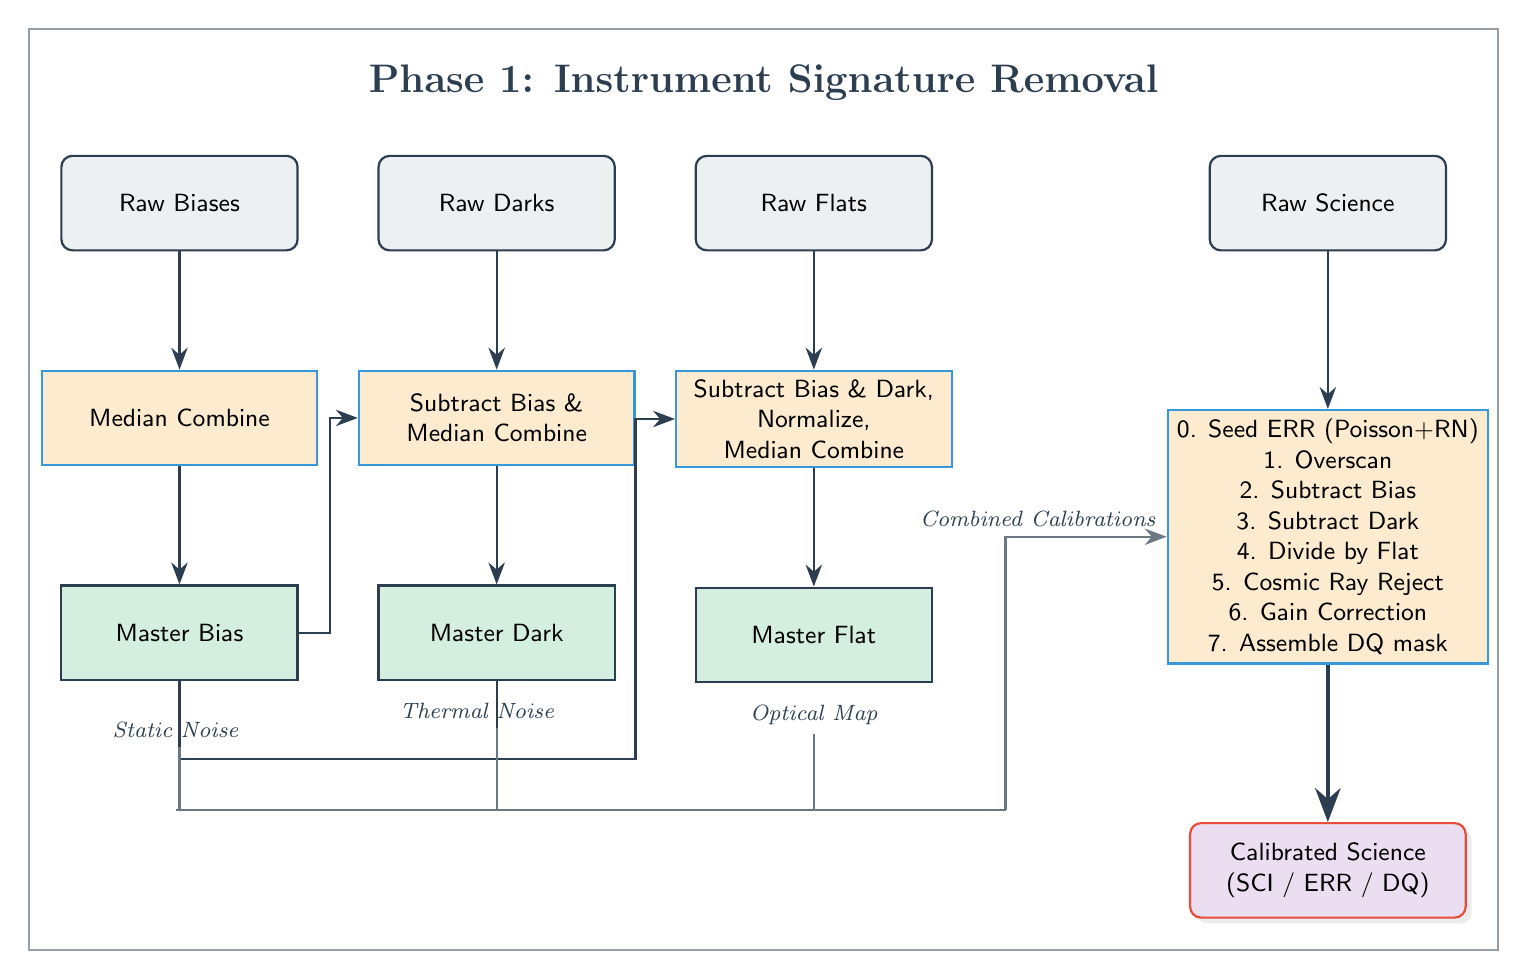
\begin{tikzpicture}[node distance=1.5cm and 1.5cm]

    % Inputs
    \node (rbias) [raw] {Raw Biases};
    \node (rdark) [raw, right=1cm of rbias] {Raw Darks};
    \node (rflat) [raw, right=1cm of rdark] {Raw Flats};
    \node (rsci)  [raw, right=3.5cm of rflat] {Raw Science};

    % Bias Process
    \node (pbias) [process, below=1.5cm of rbias] {Median Combine};
    \node (mbias) [master, below=1.5cm of pbias] {Master Bias};

    % Dark Process
    \node (pdark) [process, below=1.5cm of rdark] {Subtract Bias \&\\Median Combine};
    \node (mdark) [master, below=1.5cm of pdark] {Master Dark};

    % Flat Process 
    \node (pflat) [process, below=1.5cm of rflat] {Subtract Bias \& Dark,\\Normalize,\\Median Combine};
    \node (mflat) [master, below=1.5cm of pflat] {Master Flat};

    % Science Process
    \node (psci) [process, below=2cm of rsci] {0. Seed ERR (Poisson+RN) \\ 1. Overscan \\ 2. Subtract Bias \\ 3. Subtract Dark \\ 4. Divide by Flat \\ 5. Cosmic Ray Reject \\ 6. Gain Correction \\ 7. Assemble DQ mask};
    
    % Final Output Phase 1
    \node (calsci) [final, below=2cm of psci] {Calibrated Science\\(SCI / ERR / DQ)};

    % LABELS
    \node (lblbias) [below=0.4cm of mbias, xshift=-0.05cm, label_text] {Static Noise};
    \node (lbldark) [below=0.15cm of mdark, xshift=-0.25cm, label_text] {Thermal Noise};
    \node (lblflat) [below=0.15cm of mflat, label_text] {Optical Map};

    % Paths: Bias
    \draw [arrow] (rbias) -- (pbias);
    \draw [arrow] (pbias) -- (mbias);
    
    % Paths: Dark
    \draw [arrow] (rdark) -- (pdark);
    \draw [arrow] (mbias.east) -- ++(0.4,0) |- (pdark.west);
    \draw [arrow] (pdark) -- (mdark);

    % Paths: Flat
    \draw [arrow] (rflat) -- (pflat);
    
    % ROUTING
    \coordinate (gapPoint) at ($(mbias.east)!0.5!(mdark.west)$);
    \coordinate (dropLevel) at ($(lbldark.south) + (0, -0.4cm)$);
    \coordinate (routePoint1) at (gapPoint |- dropLevel);
    
    \coordinate (darkDropPoint) at (mdark.south |- dropLevel);
    \coordinate (flatJunct) at ($(pflat.west) + (-0.5cm, 0)$);

    \draw [thick, color=primary] (mbias.south) |- (routePoint1);
    \draw [thick, color=primary] (routePoint1) -- (darkDropPoint);
    
    \draw [thick, color=primary] (mdark.south) -- (darkDropPoint);
    
    \draw [arrow] (darkDropPoint) -| (flatJunct) -- (pflat.west);
    \draw [arrow] (pflat) -- (mflat);

    % Paths: Science
    \draw [arrow] (rsci) -- (psci);
    
    % BUS ROUTING
    \coordinate (busLevel) at ($(lblbias.south) + (0, -0.8cm)$);
    \coordinate (busRight) at ($(lblflat.east |- busLevel) + (1.5cm, 0)$);

    \draw [thick, color=primary!70] ([xshift=0.05cm]lblbias.south) -- ([xshift=0.05cm]lblbias.south |- busLevel);
    \draw [thick, color=primary!70] ([xshift=0.25cm]lbldark.south) -- ([xshift=0.25cm]lbldark.south |- busLevel);
    \draw [thick, color=primary!70] (lblflat.south) -- (lblflat.south |- busLevel);
    \draw [thick, color=primary!70] (lblbias.south |- busLevel) -- (busRight);
    
    \draw [arrow, thick, color=primary!70] (busRight) |- (psci.west) node[pos=0.60, above, label_text] {Combined Calibrations};
    
    \draw [arrow, ultra thick] (psci) -- (calsci);

    % Background Container & Centered Title
    \coordinate (topTitlePadding) at ($(rbias.north) + (0, 1.2cm)$);
    
    \begin{scope}[on background layer]
        \node [groupbox, fit=(topTitlePadding) (rbias) (rsci) (calsci) (busLevel)] (bgbox) {};
        \node [font=\Large\bfseries\color{primary}] at ([yshift=-0.7cm]bgbox.north) {Phase 1: Instrument Signature Removal};
    \end{scope}

\end{tikzpicture}
\end{center}
\end{landscape}

\newpage

\section{Phase 1: Instrument Signature Removal (ISR)}
\textbf{Core Objective:} To mathematically erase instrument-induced anomalies (static electronic noise, thermal currents, and optical defects) from raw astronomical data, outputting pristine calibrated frames --- each with a seeded \texttt{ERR} plane and a \texttt{DQ} bitmask --- ready for integration.

\subsection{Master Calibration Processes}
Phase 1 relies on constructing high Signal-to-Noise Ratio (SNR) master calibration frames using rigorous statistical rejection to prevent noise injection during science calibration. Critically, \textbf{each master frame is built \emph{with} its own uncertainty} (the standard error of the robust combine, $\mathrm{mad\_std}/\sqrt{N}$). Because \texttt{ccdproc} propagates uncertainty in quadrature through every arithmetic operation, this calibration noise automatically folds into the science frame's \texttt{ERR} plane during bias/dark subtraction and flat division.

\subsubsection{Master Bias Generation (Median Combine)}
\begin{itemize}[leftmargin=*]
    \item \textbf{Process:} The pipeline groups all raw zero-second exposure frames. These frames capture the fixed electronic readout noise floor of the sensor ("Static Noise"). 
    \item \textbf{Mathematics:} The 2D arrays are stacked into a 3D data cube. The algorithm calculates the \textbf{Median} value through the Z-axis for every $(X, Y)$ pixel coordinate. This effectively models the read-noise floor while mathematically rejecting transient anomalies like cosmic rays that only appear in a single frame.
\end{itemize}

\subsubsection{Master Dark Generation (Subtract Bias \& Median Combine)}
\begin{itemize}[leftmargin=*]
    \item \textbf{Process:} Raw dark frames capture the "Thermal Noise" that accumulates in the silicon matrix over time, even with the shutter closed.
    \item \textbf{Mathematics:} The pipeline subtracts the newly generated \textbf{Master Bias} from each individual Raw Dark frame. This ensures we are isolating purely thermal current and not double-counting read noise. The bias-subtracted darks are then median-combined along the Z-axis to reject transients, outputting the clean \textbf{Master Dark}.
\end{itemize}

\subsubsection{Master Flat Generation (Subtract, Normalize, Median Combine)}
\begin{itemize}[leftmargin=*]
    \item \textbf{Process:} Raw flats map the physical optical imperfections of the telescope (vignetting, dust donuts). 
    \item \textbf{Mathematics:} 
    \begin{enumerate}
        \item \textbf{Subtraction:} The Master Bias and Master Dark are subtracted from every raw flat to remove their electronic and thermal signatures.
        \item \textbf{Normalization:} The scalar median ADU (Analog-to-Digital Unit) value of the subtracted flat is calculated. The entire 2D matrix is then divided by this scalar value. This forces the array's average background to center around $1.0$.
        \item \textbf{Combination:} The normalized frames are median-combined, producing an "Optical Map" of percentage-based multipliers. (\textit{See \hyperref[app:flat]{Appendix A.2 for a detailed breakdown of the normalization mathematics}})
    \end{enumerate}
\end{itemize}

\subsection{The Science Processing Flow}
Raw science frames are fed through the \texttt{UniversalProcessor} and subjected to a strict sequence of mathematical corrections. The very first act is to \emph{seed} the error budget; from that point on the \texttt{ERR} plane is carried through every step automatically:
\begin{enumerate}
    \item \textbf{Error Budget Seeding:} As each raw frame is loaded, the pipeline attaches a $1\sigma$ uncertainty computed from the detector gain and read noise, $\sigma_{\mathrm{ADU}} = \sqrt{g\,I + \sigma_R^2}\,/\,g$ (Poisson photon noise plus read noise; \texttt{ccdproc.create\_deviation}). A saturation mask is also recorded from the raw ADU values for later DQ flagging. (\textit{See \hyperref[app:errbudget]{Appendix A.12}})
    \item \textbf{Overscan Correction (Conditional):} If the sensor has an unilluminated overscan region, the engine calculates the median row-by-row noise floor and subtracts it to correct for amplifier drift during readout. Because these extreme edge pixels are physically masked from light, they record the exact baseline electronic noise present at the fraction of a second that specific row is processed. Subtracting this unique median from each row completely eliminates horizontal banding caused by the camera's amplifier heating up or fluctuating during the download sequence. (\textit{See \hyperref[app:overscan]{Appendix A.3 for a deep dive into banding correction}})
    \item \textbf{Bias Subtraction:} The Master Bias (Static Noise) is subtracted from the science frame; its uncertainty adds in quadrature to the \texttt{ERR} plane.
    \item \textbf{Dark Subtraction:} The Master Dark (Thermal Noise) is subtracted from the science frame. The pipeline strictly enforces a 1:1 exposure match (\texttt{scale=False}) to preserve non-linear thermal structures. (\textit{See \hyperref[app:dark]{Appendix A.6 for the physics of dark scaling}})
    \item \textbf{Flat Division:} The image matrix is divided pixel-by-pixel by the normalized Master Flat, which mathematically brightens vignetted corners and erases dust shadows. The flat's relative uncertainty propagates into \texttt{ERR}.
    \item \textbf{Cosmic Ray Rejection:} The pipeline executes the \texttt{astroscrappy} Laplacian edge-detection algorithm. By analyzing the specific Gain and Read Noise of the camera, it differentiates legitimate point-sources (stars) from high-energy cosmic ray strikes, masking and interpolating the damaged pixels; the affected pixels are flagged in the \texttt{DQ} plane. (\textit{See \hyperref[app:cosmic]{Appendix A.4 for the underlying mathematics of the Laplacian filter}})
    \item \textbf{Gain Correction:} The final 2D matrix is multiplied by the hardware gain. This converts the data \emph{and its uncertainty} from arbitrary ADUs into true, physical Electrons ($e^-$), and the \texttt{BUNIT} FITS header is updated accordingly. (\textit{See \hyperref[app:adapter]{Appendix A.1 for how hardware metadata is safely extracted}})
    \item \textbf{DQ Assembly \& Output:} A single integer \texttt{DQ} bitmask is assembled from the saturation mask, the flat-derived Bad-Pixel Mask (BPM), the cosmic-ray mask, and any NaN/no-data pixels. The calibrated frame is written as a multi-extension FITS file with \texttt{SCI} (electrons), \texttt{ERR} ($1\sigma$), and \texttt{DQ} planes. (\textit{See \hyperref[app:bpm]{Appendix A.5 for BPM generation} and \hyperref[app:dqmask]{Appendix A.13 for the bitmask}})
\end{enumerate}

\newpage

% =========================================================
% TIKZ TREE: PHASE 2
% =========================================================
\begin{landscape}
\section{Data Flow Architecture: Phase 2 (Integration \& Astrometry)}
\vspace{1cm}

\begin{center}
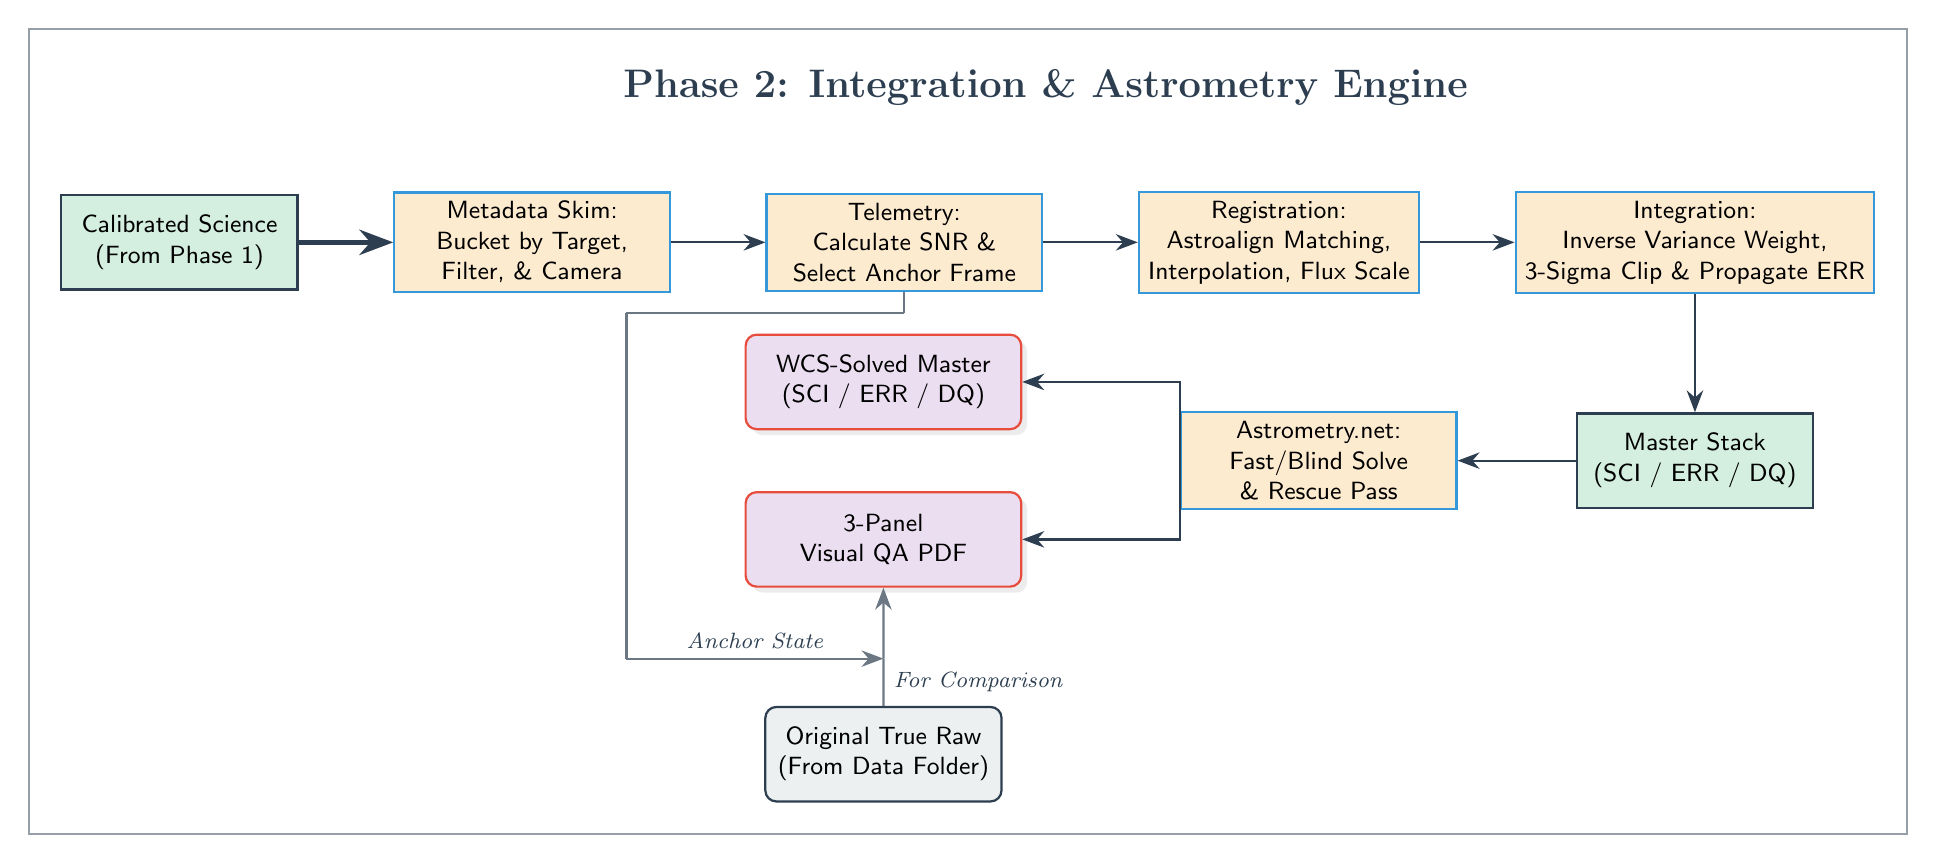
\begin{tikzpicture}[node distance=1.5cm and 1cm]

    % Phase Title
    \node (p2title) [font=\Large\bfseries\color{primary}] {Phase 2: Integration \& Astrometry Engine};

    % Phase 1 Input
    \node (incal) [master, below=1cm of p2title, xshift=-11cm] {Calibrated Science\\(From Phase 1)};

    % Grouping
    \node (group) [process, right=1.2cm of incal] {Metadata Skim:\\Bucket by Target,\\Filter, \& Camera};
    
    % Anchor Selection
    \node (anchor) [process, right=1.2cm of group] {Telemetry:\\Calculate SNR \&\\Select Anchor Frame};
    
    % Registration
    \node (reg) [process, right=1.2cm of anchor] {Registration:\\Astroalign Matching,\\Interpolation, Flux Scale};
    
    % Stacking
    \node (stack) [process, right=1.2cm of reg] {Integration:\\Inverse Variance Weight,\\3-Sigma Clip \& Propagate ERR};

    % Final Master
    \node (mstack) [master, below=1.5cm of stack] {Master Stack\\(SCI / ERR / DQ)};

    % WCS
    \node (wcs) [process, left=1.5cm of mstack] {Astrometry.net:\\Fast/Blind Solve\\\& Rescue Pass};

    % Outputs
    \node (finalfits) [final, left=2cm of wcs, yshift=1cm] {WCS-Solved Master\\(SCI / ERR / DQ)};
    \node (finalpdf)  [final, left=2cm of wcs, yshift=-1cm] {3-Panel\\Visual QA PDF};

    % External inputs for PDF
    \node (rawinput) [raw, below=1.5cm of finalpdf] {Original True Raw\\(From Data Folder)};

    % Paths: Linear Sequence
    \draw [arrow, ultra thick] (incal) -- (group);
    \draw [arrow] (group) -- (anchor);
    \draw [arrow] (anchor) -- (reg);
    \draw [arrow] (reg) -- (stack);
    \draw [arrow] (stack) -- (mstack);
    \draw [arrow] (mstack) -- (wcs);
    
    % Paths: Output Splitting
    \draw [arrow] (wcs.west) |- (finalfits.east);
    \draw [arrow] (wcs.west) |- (finalpdf.east);
    
    % Paths: PDF Data Gather 
    \coordinate (pdfJunct) at ($(rawinput.north)!0.4!(finalpdf.south)$);
    \draw [thick, color=primary!70] (rawinput) -- (pdfJunct) node[midway, right, label_text] {For Comparison};
    \draw [arrow, thick, color=primary!70] (pdfJunct) -- (finalpdf);
    
    \coordinate (midLevel) at ($(anchor.south)!0.5!(finalfits.north)$);
    \coordinate (leftOfBoxes) at ($(finalpdf.west) + (-1.5cm, 0)$);
    
    \draw [thick, color=primary!70] (anchor.south) -- (anchor.south |- midLevel);
    \draw [thick, color=primary!70] (anchor.south |- midLevel) -- (leftOfBoxes |- midLevel);
    \draw [thick, color=primary!70] (leftOfBoxes |- midLevel) -- (leftOfBoxes |- pdfJunct);
    \draw [arrow, thick, color=primary!70] (leftOfBoxes |- pdfJunct) -- (pdfJunct) node[midway, above, label_text] {Anchor State};

    % Background Container 
    \begin{scope}[on background layer]
        \node [groupbox, fit=(p2title) (incal) (group) (finalfits) (rawinput) (leftOfBoxes) (stack)] {};
    \end{scope}

\end{tikzpicture}
\end{center}
\end{landscape}
\newpage

\section{Phase 2: Integration, Astrometry \& QA Engine}
\textbf{Core Objective:} To automatically ingest Phase 1 frames, mathematically align them to a dynamic anchor, integrate them using inverse-variance weighting and sigma-clipping, and map the deep stack to true celestial coordinates.

\subsection{Grouping and Telemetry Engine}
\subsubsection{Metadata Skim (Target Grouping)}
The \texttt{FITSHandler} reads the headers of incoming calibrated science frames. It extracts the \texttt{OBJECT}, \texttt{FILTER}, and hardware metadata (focal length, pixel size). Files are dynamically bucketed into \texttt{TargetGroup} objects ensuring only data matching the exact Object/Filter/Camera combination are stacked together.

\subsubsection{Telemetry (Anchor Selection)}
Instead of randomly picking an alignment reference, the pipeline extracts a 2D background model via \texttt{photutils}. It calculates the \texttt{mad\_std} (Median Absolute Deviation) to determine the true noise floor. The single frame with the highest 99th-percentile signal divided by the lowest noise floor is crowned the \textbf{Anchor Frame}. (\textit{See \hyperref[app:mad]{Appendix A.8 for why MAD is used for noise estimation}})

\subsection{Integration Engine}
\subsubsection{Geometric Registration \& Flux Scaling}
\begin{itemize}[leftmargin=*]
    \item \textbf{Astroalign Matching:} The pipeline detects point sources and maps asterism triangles between the target frame and the Anchor frame. It solves an affine transformation matrix (Translation, Rotation, Scale). (\textit{See \hyperref[app:astroalign]{Appendix A.9 for the logic of geometric hashing}})
    \item \textbf{Interpolation:} The target image is geometrically warped to perfectly overlay the anchor using 3rd-order (bicubic) interpolation to preserve sub-pixel stellar profiles during fractional pixel shifts. (\textit{See \hyperref[app:interp]{Appendix A.7 for an explanation of sub-pixel math}})
    \item \textbf{Flux Scaling:} The \texttt{MathEngine} calculates the median flux ratio of the matched stars. The warped target is multiplied by this scalar, normalizing its brightness to match the Anchor (correcting for passing cirrus clouds or transparency loss).
    \item \textbf{Error-Plane Registration:} The \texttt{ERR} plane travels with the science data --- its variance is warped by the same transform and scaled by the square of the flux ratio ($\sigma^2 \rightarrow s^2\sigma^2$) --- so the propagated uncertainty of every pixel remains valid after alignment.
\end{itemize}

\subsubsection{Stacking (Inverse Variance Weighting \& 3-Sigma Clipping)}
\begin{itemize}[leftmargin=*]
    \item \textbf{Inverse Variance Weighting:} The noise variance of every aligned frame is calculated. Frames with lower noise are given heavier mathematical influence in the final stack; noisy frames are mathematically suppressed.
    \item \textbf{3-Sigma Clipping:} The 3D data cube undergoes Z-axis sigma-clipping. For every pixel coordinate, the algorithm computes the median and standard deviation through the stack. Any pixel deviating by more than 3-sigma (e.g., satellite trails, airplanes) is masked and rejected before the final weighted mean is computed, outputting the \textbf{Master Stack}. (\textit{See \hyperref[app:stacking]{Appendix A.10 for the mathematics of integration}})
    \item \textbf{Propagated Master \texttt{ERR}:} The variance of the weighted mean, $\mathrm{Var} = \sum w_i^2\,\sigma_i^2 / (\sum w_i)^2$ over the surviving frames, is \emph{materialized} as the master's \texttt{ERR} plane rather than merely logged. A pixel's \texttt{DQ} is flagged where no frame contributed (NaN). The historical fixed ``$+100$ ADU'' display pedestal has been removed, so the stack remains on a physical electron scale suitable for absolute photometry.
\end{itemize}

\subsection{Astrometry Engine}
\subsubsection{Plate Solving \& Rescue Pass}
\begin{itemize}[leftmargin=*]
    \item \textbf{Fast/Blind Solve:} The \texttt{WCSSolver} passes the Master Stack to the local Linux \texttt{solve-field} binary. It injects a physical \texttt{PIXSCALE} estimate (derived from focal length and pixel size) to restrict the search radius for a highly optimized "Fast Solve."
    \item \textbf{Rescue Pass:} Narrowband images (like H-Alpha) often lack enough stars to plate-solve. If a solve fails, the engine borrows the exact Right Ascension and Declination from a successfully solved filter within the same \texttt{TargetGroup}, executing a forced local search to rescue the astrometry. (\textit{See \hyperref[app:wcs]{Appendix A.11 for plate solving optimization}})
    \item \textbf{Error-Plane Preservation:} \texttt{solve-field} only understands a single-image FITS and drops extra extensions from its output. The \texttt{WCSSolver} therefore solves on the \texttt{SCI} plane, then re-attaches the \texttt{ERR} and \texttt{DQ} planes to the WCS-solved result --- so the master remains a full three-plane multi-extension file after astrometry.
\end{itemize}

\newpage

% =========================================================
% TIKZ TREE: PHASE 3
% =========================================================
\begin{landscape}
\section{Data Flow Architecture: Phase 3 (Photometry \& Zero Point)}
\vspace{1cm}

\begin{center}
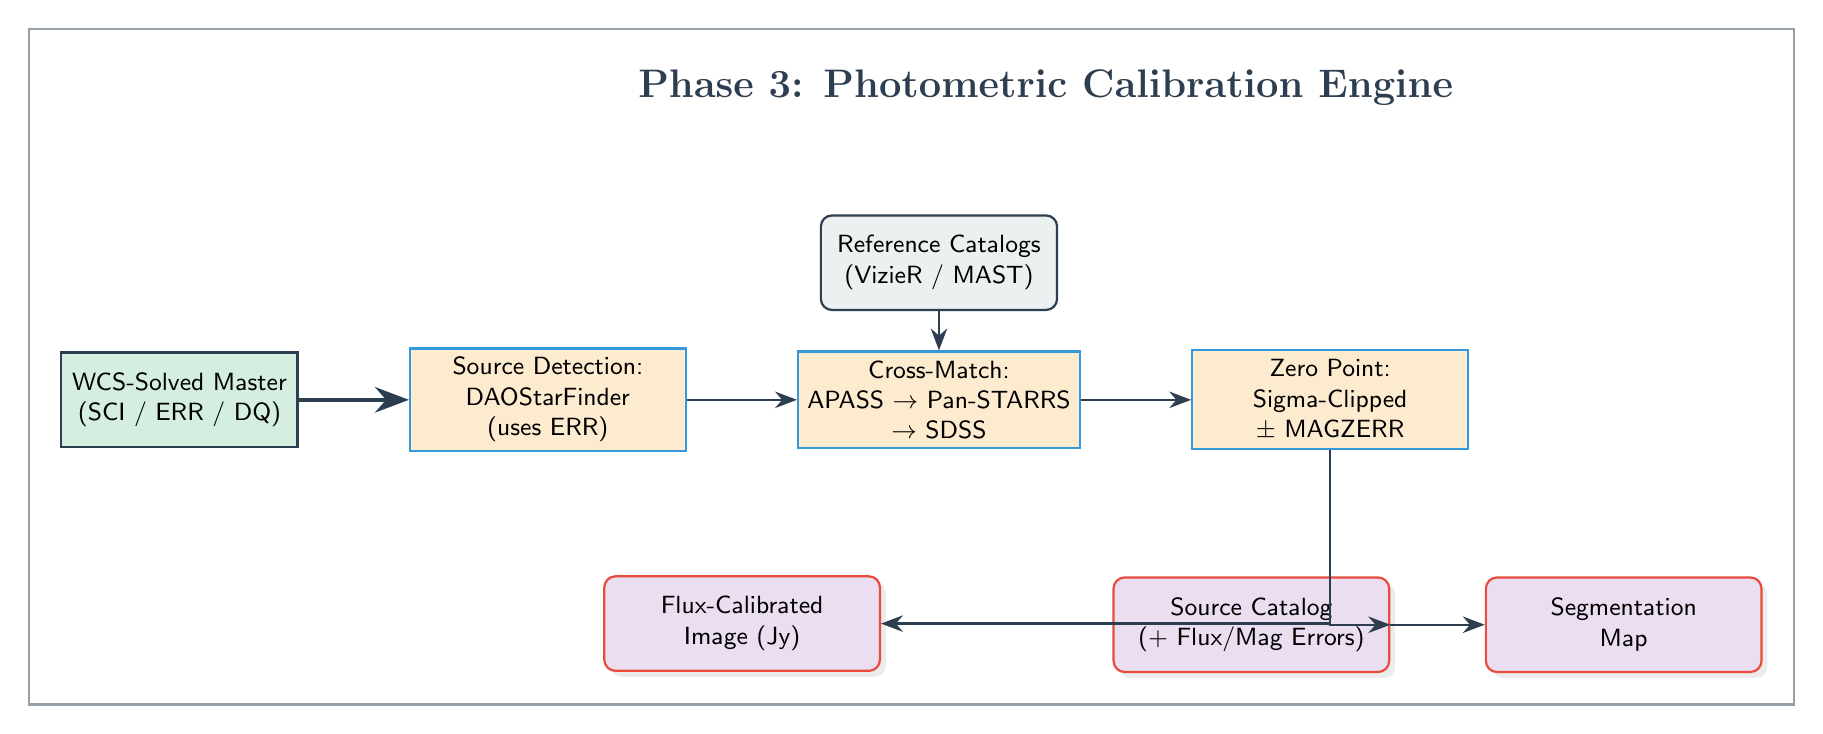
\begin{tikzpicture}[node distance=1.4cm and 1.6cm]

    \node (p3title) [font=\Large\bfseries\color{primary}] {Phase 3: Photometric Calibration Engine};

    \node (inmaster) [master, below=3cm of p3title, xshift=-11cm] {WCS-Solved Master\\(SCI / ERR / DQ)};
    \node (detect)   [process, right=1.4cm of inmaster] {Source Detection:\\DAOStarFinder\\(uses ERR)};
    \node (xmatch)   [process, right=1.4cm of detect] {Cross-Match:\\APASS $\rightarrow$ Pan-STARRS\\$\rightarrow$ SDSS};
    \node (zp)       [process, right=1.4cm of xmatch] {Zero Point:\\Sigma-Clipped\\$\pm$ MAGZERR};

    \node (fluxcal)  [final, below=1.6cm of xmatch, xshift=-2.5cm] {Flux-Calibrated\\Image (Jy)};
    \node (catalog)  [final, below=1.6cm of zp, xshift=-1cm] {Source Catalog\\(+ Flux/Mag Errors)};
    \node (segmap)   [final, right=1.2cm of catalog] {Segmentation\\Map};

    \node (refcat) [raw, above=0.5cm of xmatch] {Reference Catalogs\\(VizieR / MAST)};

    \draw [arrow, ultra thick] (inmaster) -- (detect);
    \draw [arrow] (detect) -- (xmatch);
    \draw [arrow] (xmatch) -- (zp);
    \draw [arrow] (refcat) -- (xmatch);
    \draw [arrow] (zp.south) |- (catalog.east);
    \draw [arrow] (zp.south) |- (fluxcal.east);
    \draw [arrow] (catalog) -- (segmap);

    \begin{scope}[on background layer]
        \node [groupbox, fit=(p3title) (inmaster) (refcat) (zp) (fluxcal) (segmap)] {};
    \end{scope}

\end{tikzpicture}
\end{center}
\end{landscape}
\newpage

\section{Phase 3: Photometry, Zero Point \& Catalogs}
\textbf{Core Objective:} To place the deep master stacks on a physical, filter-wise photometric scale --- deriving a zero point \emph{with a formal uncertainty}, converting pixels to Janskys, and producing a source catalogue in which every magnitude carries an error bar.

\subsection{Reference-Catalog Cross-Match}
\subsubsection{Priority Cascade}
The engine reads the WCS to convert detected star positions into sky coordinates, then queries global reference catalogues in a filter-aware priority cascade: \textbf{APASS} (Johnson $B$/$V$ and Sloan $g'/r'/i'$, ideal for small-telescope depths), falling back to \textbf{Pan-STARRS DR2} and then \textbf{SDSS DR12}. The first catalogue to return valid stars for the requested band wins, and its per-star magnitude \emph{and its uncertainty} are standardised into a common table. (\textit{See \hyperref[app:zeropoint]{Appendix A.14 for the zero-point mathematics}})

\subsection{Filter-Wise Zero Point}
\subsubsection{Differential Photometry with Uncertainty}
\begin{itemize}[leftmargin=*]
    \item \textbf{Instrumental Measurement:} For each catalogue-matched star the engine performs aperture photometry using the \texttt{ERR} plane, yielding an instrumental magnitude and its error, $\delta m_{\mathrm{inst}} = 1.0857\,\delta F / F$.
    \item \textbf{Per-Star Offset:} Each star gives a zero-point estimate $\mathrm{ZP}_i = m_{\mathrm{cat}} - m_{\mathrm{inst}}$, with an uncertainty combining the instrumental and catalogue errors in quadrature.
    \item \textbf{Robust Combination:} The per-star offsets are sigma-clipped and combined with an inverse-variance weighted mean. The pipeline records \texttt{MAGZERO}, the zero-point uncertainty \texttt{MAGZERR} (the larger of the formal weighted error and the standard error of the surviving scatter), and \texttt{NZPSTARS} in the FITS header --- one zero point per filter, each with a defensible error bar.
\end{itemize}

\subsection{Products}
\subsubsection{Flux Calibration \& Catalog}
\begin{itemize}[leftmargin=*]
    \item \textbf{Flux-Calibrated Image:} Pixels are converted to Janskys via the AB relation $F_\nu = 3631 \times 10^{-\mathrm{ZP}/2.5}$; the \texttt{ERR} plane is scaled by the same factor and preserved.
    \item \textbf{Source Catalog:} A deblended segmentation catalogue is measured with the \texttt{ERR} plane, exposing \texttt{Flux\_Error}, \texttt{Mag\_Error} $=\sqrt{(1.0857\,\delta F/F)^2 + \mathrm{MAGZERR}^2}$, \texttt{SNR}, and DQ \texttt{FLAGS} columns alongside positions, magnitudes, and shape parameters.
    \item \textbf{Verification:} The independent \texttt{cassa-verify} tool re-queries reference catalogues and reports the residual offset and scatter, confirming the reported \texttt{MAGZERR} is realistic.
\end{itemize}

\newpage

% =========================================================
% TIKZ TREE: PHASE 4
% =========================================================
\begin{landscape}
\section{Data Flow Architecture: Phase 4 (Diagnostics)}
\vspace{1cm}

\begin{center}
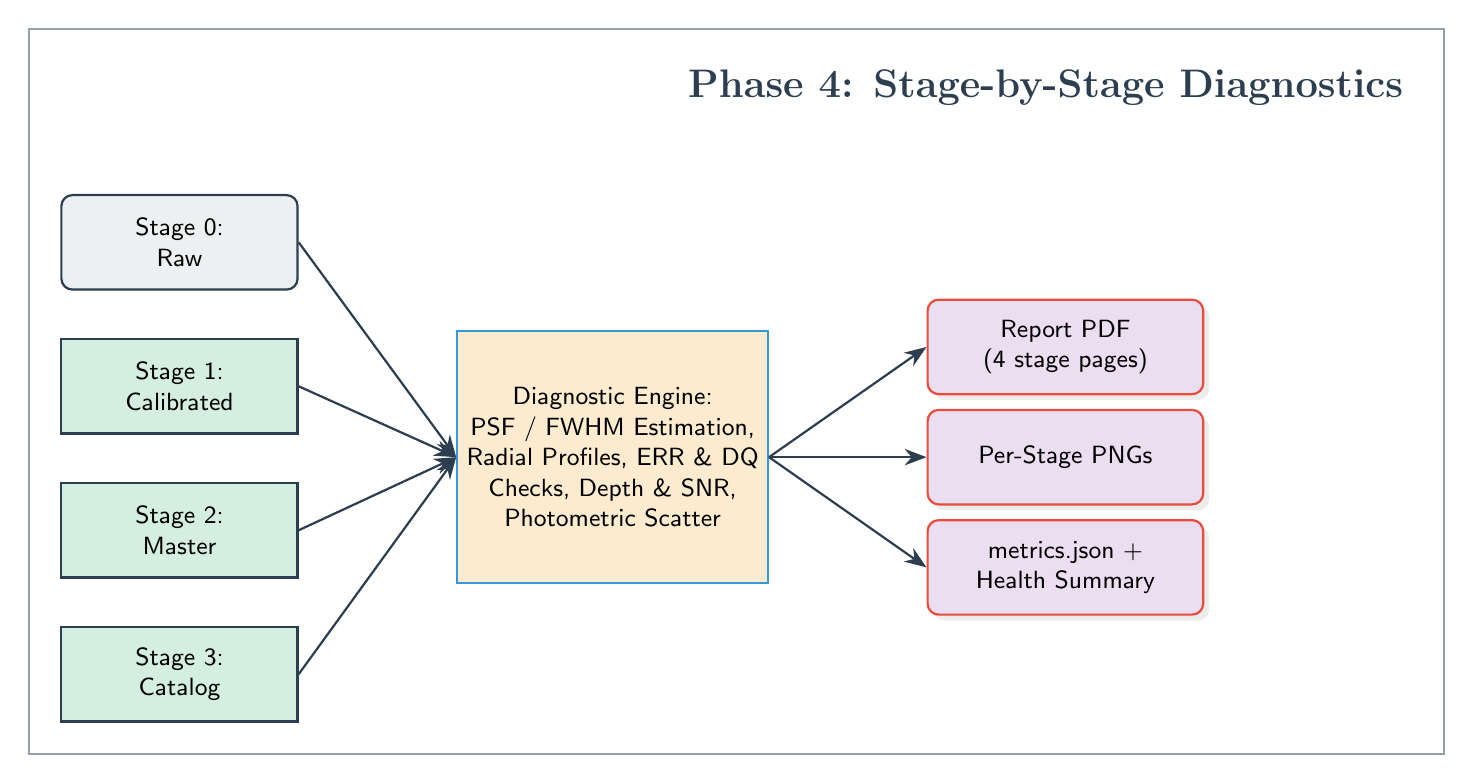
\begin{tikzpicture}[node distance=1.1cm and 1.8cm]

    \node (p4title) [font=\Large\bfseries\color{primary}] {Phase 4: Stage-by-Stage Diagnostics};

    \node (s0) [raw,    below=1cm of p4title, xshift=-11cm] {Stage 0:\\Raw};
    \node (s1) [master, below=0.6cm of s0] {Stage 1:\\Calibrated};
    \node (s2) [master, below=0.6cm of s1] {Stage 2:\\Master};
    \node (s3) [master, below=0.6cm of s2] {Stage 3:\\Catalog};

    \node (engine) [process, right=2cm of s1, yshift=-0.9cm, minimum height=3.2cm] {Diagnostic Engine:\\PSF / FWHM Estimation,\\Radial Profiles, ERR \& DQ\\Checks, Depth \& SNR,\\Photometric Scatter};

    \node (report) [final, right=2cm of engine, yshift=1.4cm] {Report PDF\\(4 stage pages)};
    \node (pngs)   [final, right=2cm of engine] {Per-Stage PNGs};
    \node (json)   [final, right=2cm of engine, yshift=-1.4cm] {metrics.json +\\Health Summary};

    \draw [arrow] (s0.east) -- (engine.west);
    \draw [arrow] (s1.east) -- (engine.west);
    \draw [arrow] (s2.east) -- (engine.west);
    \draw [arrow] (s3.east) -- (engine.west);
    \draw [arrow] (engine.east) -- (report.west);
    \draw [arrow] (engine.east) -- (pngs.west);
    \draw [arrow] (engine.east) -- (json.west);

    \begin{scope}[on background layer]
        \node [groupbox, fit=(p4title) (s0) (s3) (engine) (report) (json)] {};
    \end{scope}

\end{tikzpicture}
\end{center}
\end{landscape}
\newpage

\section{Phase 4: Diagnostics \& Validation}
\textbf{Core Objective:} To verify that the pipeline is behaving correctly at every stage, by estimating the point-spread function and producing quantitative, visual quality-assurance for the raw frame, the calibrated frame, the WCS-solved master, and the photometric catalogue.

\subsection{PSF \& Image Quality}
Across all stages, the diagnostic engine detects isolated bright stars, fits each with a 2D Gaussian, and reports a robust median \textbf{FWHM} (in pixels and, where a plate scale exists, arcseconds), an ellipticity, and a stacked \textbf{radial profile}. A stable FWHM across stages confirms that calibration and stacking have not degraded the stellar profiles. (\textit{See \hyperref[app:psf]{Appendix A.15 for the FWHM fitting method}})

\subsection{Per-Stage Checks}
\begin{itemize}[leftmargin=*]
    \item \textbf{Stage 0 (Raw):} image and histogram, background level, detected-star overlay, and a near-saturation map.
    \item \textbf{Stage 1 (Calibrated):} \texttt{SCI}/\texttt{ERR}/\texttt{DQ} panels, DQ flag counts, an \emph{error-vs-signal} (Poisson) check, and the background-flatness improvement relative to the raw frame.
    \item \textbf{Stage 2 (Master):} \texttt{SCI}/\texttt{ERR} panels and an SNR map, the depth boost relative to a single frame (the noise should drop by $\approx\!\sqrt{N}$), and the WCS status with field centre and plate scale.
    \item \textbf{Stage 3 (Photometry):} magnitude-error versus magnitude, SNR versus magnitude, number counts / limiting magnitude, a spatial source map, and a star/galaxy shape split, together with the recorded zero point and \texttt{MAGZERR}.
\end{itemize}

\subsection{Outputs}
The engine auto-discovers the products of a Phase 2 run directory (pairing them by filter) and writes a multi-page \texttt{diagnostics\_report.pdf}, per-stage PNGs, a machine-readable \texttt{metrics.json}, and a \textbf{pipeline-health summary} marking each stage \texttt{OK}, \texttt{SKIP}, or \texttt{FAIL}. Stages whose products are absent degrade gracefully rather than aborting the report.

\newpage

% =========================================================
% APPENDIX: TECHNICAL DEEP DIVES
% =========================================================
\section{Appendix: Technical Implementation Details}

\subsection{Dynamic FITS Header Extraction (The Adapter Pattern)}\label{app:adapter}
Astronomical FITS headers lack strict standardization across observatories (e.g., gain might be stored as \texttt{EGAIN}, \texttt{GAIN}, or \texttt{SYSGAIN}). To prevent pipeline crashes, Phase 1 relies on the \textbf{Adapter Pattern} via an \texttt{InstrumentProfile} class.
\begin{itemize}[leftmargin=*]
    \item \textbf{Translation Layer:} The core mathematical engine never directly reads a FITS file. Instead, it queries the \texttt{InstrumentProfile}. The profile safely iterates through known header variants to extract critical data like Gain and Read Noise.
    \item \textbf{Failsafe Fallbacks:} In the event of missing or corrupted headers, the profile utilizes a hard-coded \texttt{hardware\_database} dictionary. By extracting the telescope ID, it can safely inject verified baseline hardware constants (e.g., \texttt{'T32': \{'gain': 1.0, 'read\_noise': 9.0\}}), ensuring the processing loops never fail due to missing metadata.
\end{itemize}

\subsection{The Mathematics of Flat Frame Normalization}\label{app:flat}
Simply averaging flat frames together is mathematically dangerous, as a brighter flat frame would overpower a dimmer one, and transient anomalies (like a cosmic ray striking the flat panel) would be permanently baked into the Master Flat.
\begin{itemize}[leftmargin=*]
    \item \textbf{The Percentage Map:} By dividing every single pixel in a flat frame by that frame's overall median value, the arbitrary brightness (ADU) is converted into a percentage map centered around 1.0. A darkened corner pixel might become 0.80 (meaning 80\% transmission).
    \item \textbf{Statistical Rejection:} Once normalized, the stack of flat frames is merged using a \textbf{Median Combine} along the Z-axis. If a cosmic ray artificially spikes a pixel to a massive value in one frame, the median calculation entirely ignores it, resulting in a pristine Master Flat that solely maps permanent optical defects.
\end{itemize}

\subsection{Overscan Banding Correction}\label{app:overscan}
Amplifier heat and voltage fluctuations cause the baseline electronic noise to drift as a sensor is read out from top to bottom, resulting in horizontal banding.
\begin{itemize}[leftmargin=*]
    \item \textbf{Row-by-Row Correction:} The overscan region is a set of physical pixels explicitly covered by an opaque mask. The pipeline isolates this region and calculates a unique median noise value for \textit{each individual row} (\texttt{axis=1}). By subtracting this dynamically shifting baseline from the corresponding active pixels in that exact same row, the amplifier drift is completely mathematically flattened. 
\end{itemize}

\subsection{Laplacian Cosmic Ray Detection (\texttt{astroscrappy})}\label{app:cosmic}
The pipeline utilizes an adaptation of the L.A.Cosmic algorithm to differentiate between legitimate celestial point-sources and radiation strikes.
\begin{itemize}[leftmargin=*]
    \item \textbf{Second Derivative Filter:} Legitimate stars possess a Point Spread Function (PSF)—their light blurs across multiple pixels in a smooth Gaussian curve. Cosmic rays impact the silicon directly, creating an infinitely sharp, single-pixel spike. The pipeline applies a \textbf{Laplacian filter} (calculating the second derivative of brightness), which measures the \textit{sharpness} of the data. 
    \item \textbf{Physics-Based Thresholding:} The algorithm is fed the specific \texttt{EGAIN} and \texttt{READNOISE} of the camera to establish the true statistical noise floor. If a pixel's Laplacian sharpness exceeds a strict threshold (e.g., 4.5$\sigma$ above the noise limit), it is mathematically proven to be a cosmic ray. The pixel is masked, and its value is interpolated from surrounding healthy pixels.
\end{itemize}

\subsection{Bad Pixel Mask Generation (BPM)}\label{app:bpm}
While cosmic rays are transient anomalies, camera sensors also suffer from permanent hardware defects, such as "dead" pixels (always read zero) or "hot" pixels (always read maximum signal).
\begin{itemize}[leftmargin=*]
    \item \textbf{Derivation from Flats:} The pipeline \emph{generates} the Bad Pixel Mask directly from the normalised master flats: any pixel whose response deviates strongly from unity (by default, below $0.5\times$ or above $1.5\times$ the median), or which is non-finite, is flagged as defective. Pooling this across all filters yields a robust, detector-level BPM.
    \item \textbf{Folded into DQ:} Rather than silently discarding these pixels, the BPM is recorded in the \texttt{DQ} bitmask (bit 2, \texttt{BAD\_PIXEL}) so that downstream stages can see, and choose how to treat, every flagged coordinate.
\end{itemize}

\subsection{Strict Dark Current Matching vs. Scaling}\label{app:dark}
Astronomical thermal noise is notoriously complex. While baseline dark current accumulates somewhat linearly over time, other thermal artifacts do not.
\begin{itemize}[leftmargin=*]
    \item \textbf{The Scaling Problem:} Modern CMOS sensors (and many CCDs) exhibit "amplifier glow"—a localized thermal bloom near the sensor's electronics. This glow is highly non-linear. If the pipeline were to mathematically scale a 300-second dark frame by a factor of 2 to calibrate a 600-second science frame, it would severely over-correct the amplifier glow, creating black holes in the final image.
    \item \textbf{The \texttt{scale=False} Imperative:} By explicitly setting \texttt{scale=False} during the \texttt{subtract\_dark} operation, the pipeline enforces strict rigor: it refuses to scale thermal frames. It mandates that the Master Dark exposure time must perfectly match the science frame exposure time, preserving the non-linear thermal structures and ensuring a mathematically perfect subtraction.
\end{itemize}

\subsection{Sub-Pixel Interpolation Physics}\label{app:interp}
When aligning multiple astronomical exposures, stars never land on the exact same physical pixels due to atmospheric turbulence or mechanical tracking errors. To correct for these fractional shifts (e.g., sliding an image by 0.4 pixels), the pipeline must mathematically guess the new grid values.
\begin{itemize}[leftmargin=*]
    \item \textbf{The Danger of Low-Order Math:} A star's light spreads across pixels in a smooth Gaussian bell curve. Using 1st-Order (Bilinear) interpolation essentially draws straight lines between neighboring pixels. During a sub-pixel shift, this straight-line math literally cuts off the peak of the star's bell curve, resulting in a blunt profile and a permanent loss of scientific flux data.
    \item \textbf{3rd-Order Preservation:} By calculating smooth, 3rd-order polynomial curves across a 4x4 grid of neighboring pixels, the bicubic interpolation algorithm perfectly recreates the natural, curved slope of the star. This allows the pipeline to slide images by microscopic fractions of a pixel while mathematically preserving the exact shape and peak brightness of the astronomical data.
\end{itemize}

\subsection{Robust Noise Estimation (Median Absolute Deviation)}\label{app:mad}
When selecting the best Anchor frame, the pipeline must calculate the Signal-to-Noise Ratio (SNR) of every image. However, calculating standard deviation on an astronomical image is dangerous because bright stars and cosmic rays artificially inflate the variance.
\begin{itemize}[leftmargin=*]
    \item \textbf{MAD vs. Standard Deviation:} Instead of standard deviation, the pipeline uses the Median Absolute Deviation (\texttt{mad\_std}). MAD calculates the median of the data, subtracts that median from every pixel, and then finds the median of those absolute differences. This makes the noise floor calculation entirely immune to bright outlier pixels, providing a mathematically pure representation of the true background sky noise.
\end{itemize}

\subsection{Asterism Geometric Hashing (Astroalign)}\label{app:astroalign}
Professional pipelines cannot rely on FITS header coordinates (WCS) for alignment because telescopes suffer from mechanical flexure, tracking drift, and meridian flips.
\begin{itemize}[leftmargin=*]
    \item \textbf{Triangle Invariance:} The \texttt{astroalign} algorithm extracts the brightest stars in an image and forms them into sets of triangles (asterisms). The internal angles of a triangle never change, regardless of whether the image is translated, scaled, or rotated $180^\circ$. By cross-matching these triangle ratios between the Target and the Anchor, the pipeline can blindly calculate a perfect affine transformation matrix without needing any telescope telemetry.
\end{itemize}

\subsection{Integration Mathematics (Weighting \& Clipping)}\label{app:stacking}
Combining the aligned images requires protecting the stack from transient events (satellites) and varying atmospheric conditions (passing clouds).
\begin{itemize}[leftmargin=*]
    \item \textbf{Inverse Variance Weighting:} Not all frames are equal. A frame taken through thin cirrus clouds will have higher noise. The pipeline assigns a weight to each pixel equal to $1/\sigma^2$. This ensures pristine frames mathematically dominate the final stack, while noisy frames contribute proportionally less, maximizing the final SNR.
    \item \textbf{Z-Axis Sigma Clipping:} To erase satellite trails, the algorithm looks "down" through the stack of aligned images at a specific $(X,Y)$ coordinate. It calculates the median and standard deviation of that specific pixel column. If a satellite crossed that pixel in frame 4, its value will spike $>3\sigma$ above the median. The algorithm mathematically masks that outlier before calculating the final weighted average.
\end{itemize}

\subsection{Blind Plate Solving Optimization}\label{app:wcs}
Astrometry.net maps pixels to physical sky coordinates (Right Ascension / Declination) by comparing star patterns to a global index.
\begin{itemize}[leftmargin=*]
    \item \textbf{Speeding up the Blind Solve:} A true "blind" solve searches the entire sky at every possible magnification scale, which is computationally expensive. The pipeline extracts the camera's pixel size and telescope focal length from the FITS header to calculate a physical \texttt{PIXSCALE} (arcseconds per pixel). Injecting this constraint restricts the solver's search radius, turning a 5-minute blind solve into a 5-second localized solve.
\end{itemize}

\subsection{Seeding the Error Budget (\texttt{create\_deviation})}\label{app:errbudget}
The single most important step for producing science-grade uncertainties is to establish a physically correct error at the very start, before any subtraction can hide it.
\begin{itemize}[leftmargin=*]
    \item \textbf{The CCD Noise Equation:} A raw pixel's variance is the sum of two independent physical sources: Poisson (shot) noise from the arriving photons, which in electrons equals the signal itself, and the fixed read noise of the amplifier. Working in ADU with gain $g$ ($e^-$/ADU) and read noise $\sigma_R$ ($e^-$), the per-pixel $1\sigma$ deviation is $\sigma_{\mathrm{ADU}} = \sqrt{g\,I + \sigma_R^2}\,/\,g$.
    \item \textbf{Automatic Propagation:} Once this uncertainty is attached (\texttt{ccdproc.create\_deviation}), every subsequent \texttt{ccdproc} operation --- bias subtraction, dark subtraction, flat division, gain correction --- combines it in quadrature with the master frames' own uncertainties, so no bespoke error bookkeeping is required. Gain correction multiplies both the data and its uncertainty by $g$, converting the whole budget from ADU to electrons.
\end{itemize}

\subsection{The Data-Quality Bitmask (DQ)}\label{app:dqmask}
Rather than deleting or interpolating away suspect pixels invisibly, the pipeline records \emph{why} each pixel is suspect in an integer bitmask, so downstream code can make its own decisions.
\begin{itemize}[leftmargin=*]
    \item \textbf{Independent Bits:} Each condition owns one bit --- \texttt{SATURATED} (1), \texttt{BAD\_PIXEL} (2), \texttt{COSMIC\_RAY} (4), \texttt{NO\_DATA} (8) --- so multiple conditions can coexist on the same pixel via a bitwise OR. A pixel flagged \texttt{5} is both saturated and a cosmic-ray hit.
    \item \textbf{Propagation:} The \texttt{DQ} plane travels with \texttt{SCI}/\texttt{ERR} through stacking and photometry. In the source catalogue, the \texttt{FLAGS} column reports the OR of all \texttt{DQ} bits falling within each source's segment, so a user can trivially reject, say, any source touching a saturated or bad pixel.
\end{itemize}

\subsection{Filter-Wise Zero Point with Uncertainty}\label{app:zeropoint}
A zero point translates instrumental magnitudes onto a standard system; reporting it \emph{without} an uncertainty makes every downstream magnitude untrustworthy.
\begin{itemize}[leftmargin=*]
    \item \textbf{Per-Star Estimates:} Each catalogue-matched star yields $\mathrm{ZP}_i = m_{\mathrm{cat}} - m_{\mathrm{inst}}$. Because the instrumental measurement uses the \texttt{ERR} plane, each estimate carries its own uncertainty $\sqrt{\delta m_{\mathrm{inst}}^2 + \delta m_{\mathrm{cat}}^2}$, where the magnitude error relates to the fractional flux error by the Pogson factor $\delta m = 1.0857\,\delta F/F$.
    \item \textbf{Robust Combination:} The set of $\mathrm{ZP}_i$ is sigma-clipped to reject mismatches and variables, then combined as an inverse-variance weighted mean. The reported \texttt{MAGZERR} is the larger of the formal weighted error $\sqrt{1/\sum w_i}$ and the standard error of the surviving scatter $\sigma/\sqrt{N}$ --- a deliberately conservative choice that captures both measurement precision and real field-to-field spread.
\end{itemize}

\subsection{PSF Estimation via 2D Gaussian Fitting}\label{app:psf}
The full-width at half-maximum (FWHM) of stars is the single most informative image-quality metric, tracking seeing, focus, and tracking errors.
\begin{itemize}[leftmargin=*]
    \item \textbf{Star Selection:} The engine detects sources, then keeps only isolated, non-edge, unsaturated stars (a saturated star has a flat top --- many pixels sharing the peak value --- and is rejected). This prevents blends and saturated cores from biasing the measurement.
    \item \textbf{Fitting \& Robust Median:} Each selected star is fit with a 2D Gaussian plus a constant background; the FWHM follows from the fitted standard deviations as $2\sqrt{2\ln 2}\,\sigma$, and the axis ratio yields an ellipticity. The per-star FWHMs are sigma-clipped and the median is reported, while the peak-normalised cutouts are stacked into a mean radial profile for visual inspection.
\end{itemize}

\newpage

% =========================================================
% PART IV: DIMM SEEING MONITOR
% =========================================================
\part*{Part IV: Atmospheric Seeing Monitor}
\addcontentsline{toc}{part}{Part IV: Atmospheric Seeing Monitor (cassa-dimm)}

\section{DIMM Overview \& Deployment}
The \texttt{cassa-dimm} package is a professional \textbf{Differential Image Motion Monitor (DIMM)}: a continuous atmospheric-seeing monitor that runs alongside the imaging pipeline. It drives an 8-inch SkyWatcher on an EQ6R-Pro fitted with a two-hole aperture mask, one hole carrying a wedge prism, so that every star produces \emph{two} spots on the detector. By tracking how the separation between the two spots jitters from frame to frame, the pipeline measures the Fried parameter $r_0$ and reports the seeing --- independently of telescope tracking errors, which cancel in the differential measurement.

\subsection{Principle of Operation}
A single-aperture image dances on the detector under atmospheric turbulence (and mount tracking error). Because both prism spots are formed by the \emph{same} telescope, any motion common to both --- tracking drift, wind shake, overall image wander --- cancels when we look at the \textbf{difference} of the two centroids. What remains is the differential wavefront tilt between the two mask sub-apertures, whose variance is a clean, calibratable measure of the turbulence integrated along the line of sight. The variance is converted to $r_0$ and then to a seeing FWHM. (\textit{See \hyperref[app:dimmphys]{Appendix B.1}})

\subsection{Installation}
The DIMM pipeline shares the same Conda environment as the imaging pipeline (Part II); only the package itself needs to be installed:
\begin{lstlisting}[language=bash]
conda activate pipeline_env
cd DIMM
pip install -e . --no-deps --no-build-isolation
\end{lstlisting}
This registers three commands:
\begin{center}
\begin{tabularx}{\textwidth}{|l|X|}
\hline
\textbf{Command} & \textbf{Role} \\
\hline
\texttt{cassa-dimm-monitor} & Continuous watch-folder seeing monitor (the production tool) \\
\hline
\texttt{cassa-dimm-batch} & One-shot reduction of a FITS cube or a folder of frames \\
\hline
\texttt{cassa-dimm-sim} & Generate synthetic frames with a known injected seeing (testing) \\
\hline
\end{tabularx}
\end{center}

\subsection{Running the Monitor}
The acquisition script on the telescope server streams individual FITS frames into a watched folder. The monitor keeps a rolling window of the most recent frames and emits a fresh seeing estimate every few seconds. Copy and edit the example configuration first --- in particular the \textbf{site latitude/longitude} (required for the airmass correction) and the watch folder:
\begin{lstlisting}[language=bash]
cp config.example.yaml config.yaml     # set site coords + watch folder
cassa-dimm-monitor --config config.yaml --folder /path/to/watch_folder
\end{lstlisting}
Every measurement is written to the output directory:
\begin{center}
\begin{tabularx}{\textwidth}{|l|X|}
\hline
\textbf{File} & \textbf{Contents} \\
\hline
\texttt{seeing\_log.csv} / \texttt{.jsonl} & Time series: timestamp, seeing (zenith \& raw), longitudinal/transverse, $r_0$, airmass, N frames, N stars, star scatter, SNR, QC flags \\
\hline
\texttt{status\_latest.json} & The latest measurement, for an observatory dashboard to poll \\
\hline
\texttt{seeing\_timeseries.png} & A live seeing-versus-time plot \\
\hline
\end{tabularx}
\end{center}

\subsection{Trying It with Simulated Data}
Before any real data is available, the whole chain can be exercised with the
built-in simulator, which injects a \emph{known} seeing so the result can be
checked. The quickest test is a one-shot batch reduction:
\begin{lstlisting}[language=bash]
# Generate 500 frames with an injected seeing of 1.5" (3 star doublets)
cassa-dimm-sim --out /tmp/dimm_demo --seeing 1.5 --nstars 3 --frames 500

# Reduce them -> should report ~1.5" with stars=3
cassa-dimm-batch /tmp/dimm_demo
#   Seeing (zenith): 1.46" +/- 0.05 | raw=1.45" | r0=6.9 cm | stars=3 | flags=[]
\end{lstlisting}

To exercise the \emph{continuous} monitor and watch the outputs build up, point
it at a folder and let frames appear there. In production the acquisition server
streams frames into this folder; for a demo you can pre-fill it (and set
\texttt{watch.process\_existing: true}), or copy frames in a few batches to see
the time series grow:
\begin{lstlisting}[language=bash]
mkdir -p /tmp/dimm_watch /tmp/dimm_out
cassa-dimm-monitor --config config.yaml --folder /tmp/dimm_watch --outdir /tmp/dimm_out &

# Feed simulated frames into the watched folder (repeat, or copy in batches)
cassa-dimm-sim --out /tmp/dimm_watch --seeing 1.5 --nstars 3 --frames 600
\end{lstlisting}
Then inspect \texttt{/tmp/dimm\_out}: \texttt{status\_latest.json} holds the most
recent seeing, \texttt{seeing\_log.csv} accumulates the time series, and
\texttt{seeing\_timeseries.png} is the live plot. A healthy run reports the
longitudinal and transverse seeing in agreement and recovers the injected value.

\begin{landscape}
\section{Data Flow Architecture: DIMM Seeing Monitor}
\vspace{1cm}

\begin{center}
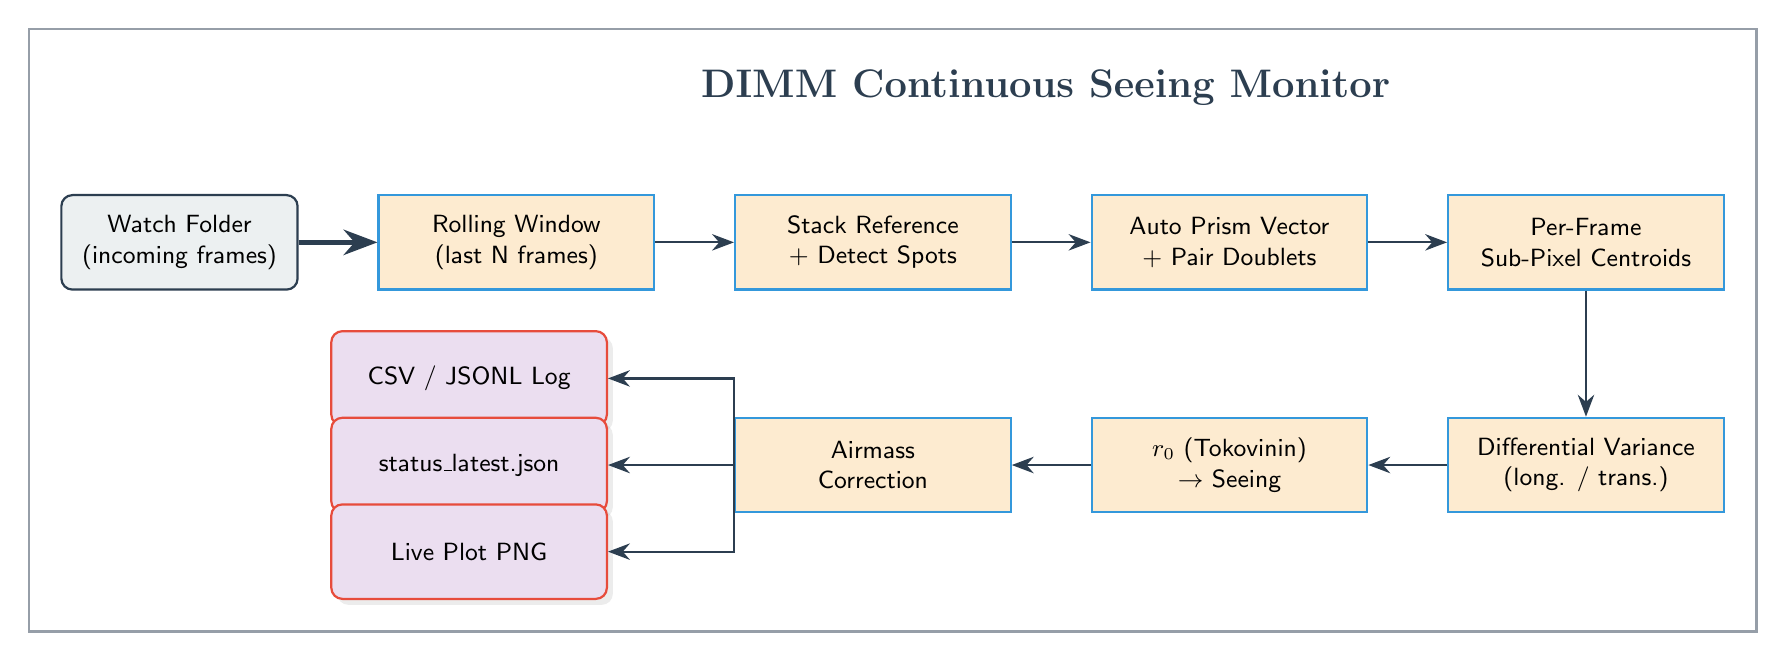
\begin{tikzpicture}[node distance=0.9cm and 1.0cm]

    \node (title) [font=\Large\bfseries\color{primary}] {DIMM Continuous Seeing Monitor};

    % Row 1 (left to right)
    \node (watch) [raw, below=1cm of title, xshift=-11cm] {Watch Folder\\(incoming frames)};
    \node (win)   [process, right=of watch] {Rolling Window\\(last N frames)};
    \node (det)   [process, right=of win] {Stack Reference\\+ Detect Spots};
    \node (pair)  [process, right=of det] {Auto Prism Vector\\+ Pair Doublets};
    \node (cen)   [process, right=of pair] {Per-Frame\\Sub-Pixel Centroids};

    % Row 2 (right to left)
    \node (var)   [process, below=1.6cm of cen] {Differential Variance\\(long. / trans.)};
    \node (see)   [process, left=of var] {$r_0$ (Tokovinin)\\$\rightarrow$ Seeing};
    \node (air)   [process, left=of see] {Airmass\\Correction};

    % Outputs
    \node (out1)  [final, left=1.6cm of air, yshift=1.1cm] {CSV / JSONL Log};
    \node (out2)  [final, left=1.6cm of air] {status\_latest.json};
    \node (out3)  [final, left=1.6cm of air, yshift=-1.1cm] {Live Plot PNG};

    % Arrows
    \draw [arrow, ultra thick] (watch) -- (win);
    \draw [arrow] (win) -- (det);
    \draw [arrow] (det) -- (pair);
    \draw [arrow] (pair) -- (cen);
    \draw [arrow] (cen) -- (var);
    \draw [arrow] (var) -- (see);
    \draw [arrow] (see) -- (air);
    \draw [arrow] (air.west) |- (out1.east);
    \draw [arrow] (air.west) |- (out2.east);
    \draw [arrow] (air.west) |- (out3.east);

    \begin{scope}[on background layer]
        \node [groupbox, fit=(title) (watch) (cen) (var) (out1) (out3)] {};
    \end{scope}

\end{tikzpicture}
\end{center}
\end{landscape}
\newpage

\section{DIMM Reduction Engine}
\textbf{Core Objective:} To turn a rolling stream of short-exposure frames --- each showing every star twice --- into a robust, airmass-corrected seeing value, using \emph{all} the stars in the field for the best possible statistics.

\subsection{Multi-Star Detection \& Doublet Pairing}
Unlike a classic single-star DIMM, the field may contain several stars, each split into a doublet by the prism.
\begin{itemize}[leftmargin=*]
    \item \textbf{Stacked Reference:} The frames in the current window are mean-combined into a high-SNR reference; \texttt{DAOStarFinder} then detects all spots on it.
    \item \textbf{Prism-Vector Auto-Calibration:} The prism shifts every star's second image by the \emph{same} fixed vector. The engine histograms all pairwise spot offsets; the one repeated offset that many pairs share is the prism doublet vector. (A known value can be pinned in the config instead.)
    \item \textbf{Pairing:} Spots are greedily paired --- brightest first --- into doublets matching that vector, rejecting blends, saturated cores, and edge sources. Each surviving doublet's two reference positions are then tracked frame-to-frame.
\end{itemize}

\subsection{Sub-Pixel Centroiding}
For each spot in each frame the engine cuts a small window around the reference position, applies a 3$\times$3 median despike and local-background subtraction, and computes a centre-of-mass centroid. A \textbf{second pass re-centres the window on the first-pass centroid}, which removes the inward bias that common tracking motion would otherwise introduce by clipping a spot's wings --- a correction that materially improves accuracy. (\textit{See \hyperref[app:twopass]{Appendix B.2}})

\subsection{Seeing Physics}
For each doublet the per-frame separation $(x_1-x_2,\,y_1-y_2)$ is rotated into a \textbf{longitudinal} component (along the doublet vector) and a \textbf{transverse} component (perpendicular to it), and each is sigma-clipped to reject cloud/glitch frames. Their variances $\sigma_l^2,\sigma_t^2$ (converted to rad$^2$ via the plate scale) give the Fried parameter through the Sarazin \& Roddier (1990) / Tokovinin (2002) relations, with $D$ the sub-aperture diameter and $d$ the hole separation:
\begin{align*}
\sigma_l^2 &= 2\,\lambda^2\, r_0^{-5/3}\, c_l, & c_l &= 0.179\,D^{-1/3} - 0.0968\,d^{-1/3} \\
\sigma_t^2 &= 2\,\lambda^2\, r_0^{-5/3}\, c_t, & c_t &= 0.179\,D^{-1/3} - 0.145\,d^{-1/3}
\end{align*}
$$ r_0 = \left(\frac{2\,\lambda^2\, c}{\sigma^2}\right)^{3/5}, \qquad \varepsilon_0 = 0.98\,\frac{\lambda}{r_0} \;\text{(FWHM)}. $$
The longitudinal and transverse estimates are computed separately; their agreement is a built-in sanity check (a large discrepancy flags wind shake or tracking problems).

\subsection{Airmass Correction \& Multi-Star Combination}
\begin{itemize}[leftmargin=*]
    \item \textbf{To the Zenith:} Turbulence is measured along a slanted line of sight, so seeing worsens with airmass. The engine computes the target altitude from the header RA/Dec, the observation time, and the configured site (via \texttt{astropy} \texttt{AltAz}), forms the airmass $X$ (Kasten \& Young 1989), and corrects to the zenith: $\varepsilon_0 = \varepsilon\,X^{-0.6}$.
    \item \textbf{Combining Stars:} Every valid doublet yields an independent seeing estimate; these are combined with an SNR weighting for the final value, and the \textbf{star-to-star scatter} is reported as a quality metric. Using many doublets sharply improves the statistical precision and cadence over a single star.
\end{itemize}

\subsection{Continuous Monitoring \& Quality Control}
A stdlib polling watcher scans the folder, deferring any file whose modification time is too recent (still being written) and catching up on a backlog quickly. Each frame is reduced \emph{as it arrives} (see Wide-Field Operation below), and every \emph{cadence} frames the monitor appends a timestamped record to the logs, refreshes the live plot, and rewrites \texttt{status\_latest.json}. Each window is flagged with the reasons it passed or failed: too few frames or doublets, low valid-frame fraction, longitudinal/transverse disagreement, or a missing airmass. Bad windows are recorded but do not corrupt the trend.

\subsection{Wide-Field Operation (0.5$^\circ$ Fields)}
The 8-inch camera delivers a wide field (about half a degree, thousands of pixels across). Three features make this practical:
\begin{itemize}[leftmargin=*]
    \item \textbf{Stamp buffering (bounded memory):} Rather than buffering a window of full frames --- which for a 0.5$^\circ$ field would be gigabytes --- the monitor processes each frame on arrival. It keeps a single exponential-moving-average reference for detection and, per doublet, only a rolling deque of the differential offsets. Memory is therefore $\sim$one frame regardless of the window length or field size; in tests, streaming 180 frames of $1500\times1500$ grew memory by $\sim$0.1~GB where a full-frame buffer would have needed $\sim$1.35~GB.
    \item \textbf{Ellipticity rejection:} A fast $f/5$ Newtonian has real coma off-axis. Each detected spot's ellipticity is measured from its second moments, and spots more elongated than a configurable limit are rejected, so aberrated field-edge stars do not degrade the result.
    \item \textbf{Central-field restriction:} Optionally, only stars within a configurable radius (in arcminutes) of the field centre are used --- a simple way to confine the measurement to the best-corrected part of the field while still averaging many doublets.
\end{itemize}
Because many stars across the field each yield an independent seeing estimate, a wide field is a statistical advantage: the values are combined for precision, and their scatter is reported as a quality metric.

\section{Appendix: DIMM Technical Details}

\subsection{Differential Image Motion \& the Fried Parameter}\label{app:dimmphys}
The Fried parameter $r_0$ is the diameter over which the atmospheric wavefront stays roughly coherent; larger $r_0$ means better seeing. A single aperture's image position wanders with the wavefront tilt averaged over that aperture, but this includes telescope tracking motion that we cannot separate from the atmosphere.
\begin{itemize}[leftmargin=*]
    \item \textbf{Why Differential:} Two sub-apertures on the same telescope see the same tracking motion but statistically independent atmospheric tilts. Subtracting their centroids cancels the common motion exactly, leaving a differential variance that depends only on the turbulence and the fixed geometry $(D,d)$ --- which is why a DIMM needs no absolute pointing stability, only that both spots stay on the detector.
    \item \textbf{Two Axes:} The longitudinal (baseline-parallel) and transverse variances have different coefficients because turbulence correlates differently along and across the sub-aperture baseline; measuring both provides two independent seeing values and a consistency check.
\end{itemize}

\subsection{Two-Pass Centroiding Against Tracking Motion}\label{app:twopass}
A fixed measurement window centred on a spot's mean position is dangerous: when common tracking motion carries the spot toward the edge of its window, the far wing of the point-spread function is clipped and the centre-of-mass is pulled \emph{inward}. Because both spots suffer this pull, the measured differential motion is damped and the seeing is biased artificially good.
\begin{itemize}[leftmargin=*]
    \item \textbf{The Fix:} The engine centroids once to locate the spot, then re-extracts the window centred on that first estimate and centroids again. The spot is now centred in its own window regardless of where common motion carried it, so the full PSF is captured and the differential motion --- and hence the seeing --- is recovered without bias.
\end{itemize}

\end{document}